\documentclass{beamer}

\usetheme{CambridgeUS}
\usepackage{graphicx}
\usepackage{caption}
\usepackage{subcaption}
\usepackage{listings}
\usepackage{amsmath}
\usepackage{mathtools}
\usepackage{algorithm}
\usepackage{algorithmic}

\usepackage[framed,numbered,autolinebreaks,useliterate]{mcode}



\usepackage[style=authoryear]{biblatex}
\bibliography{hmm}

\title[ARIA]{Hidden Markov Models}

\subtitle{From Theory to Applications}

\author[A. Sorici, T. Berariu]{Alexandru Sorici, Tudor Berariu}

\institute[AI-MAS]{Romanian Asociation for Artificial Intelligence}

\date{October, 27$^{\text{th}}$, 2012}


%% TODO de pus frumos titlurile secțiunilor

%% Autori: Alexandru Sorici, Tudor Berariu
%% Data: Noiembrie 2012

\titlegraphic{
  
\includegraphics[height=.25\textheight]{graphics/branding/aria-logo-small-white.png}
}

%% Numele algoritmului
\floatname{algorithm}{Algoritmul}

%% comandă care trage o linie orizontală (80% din spațiu)
\newcommand{\horiline}{
  \vspace*{-.75em} \begin{center} \begin{tabularx}{.8\linewidth}{
        l } \hline
    \end{tabularx}
  \end{center}
  \vspace*{-.75em}
}

%% comandă pentru frame-uri goale
\newcommand{\dummyframe}{
  \begin{frame}
    \frametitle{De înlocuit} 
    :) 
  \end{frame}
}


%% afișează cuprinsul înainte de fiecare subsecțiune
\AtBeginSubsection[] {
  %\renewcommand\Switch{0}
  \begin{frame}{Outline}
    \tableofcontents[currentsection,currentsubsection,hideallsections]
  \end{frame}
  %\renewcommand\Switch{1}
}



\begin{document}
\maketitle

\begin{frame}
  \tableofcontents[onlyparts]
\end{frame}

\begin{frame}
  \frametitle{Outline}
  \tableofcontents[pausesections]
\end{frame}



\part{Intro}

\section{ARIA Education Workshops}
\label{sec:aria}

%% TODO: de luat de la Andreea Ciortea

\subsection{ARIA's Mission}
\label{sec:arimamis}

%% TODO: de luat de la Andreea Ciortea

\subsection{ARIA Education}
\label{sec:ae}

%% TODO: de luat de la Andreea Ciortea

\begin{frame}
  \frametitle{ARIA EDU} :)
\end{frame}

\subsection{Workshop Program}
\label{sec:program}
%% TODO: program pe ore (nu cu topics de discutat, ci mai degraba cu
%% time split)
\begin{frame}
  \frametitle{Today's Program}

  \begin{table}[h]
    \centering
    \begin{tabular}{|| l | l ||}
      \hline \hline
      9:00 & Registration \\
      \hline
      10:00 & ARIA \\
      \hline \hline
      11:00 & HMM Theory \\
      \hline \hline
      
    \end{tabular}
    % \caption{Today's Program}
    \label{tab:program}
  \end{table}
\end{frame}

\part{Theory of HMMs}


\section{Machine Learning Applications for HMM}
\label{sec:ml}

% introducere in invatare automata + categorisire probleme
\subsection{Machine Learning}
\label{sec:hmm_in_ml}

\begin{frame}
  \frametitle{What is Machine Learning?}
  \begin{block}{Machine Learning}
    ..\alert{Trascau} is a beautiful horse.
  \end{block}
\end{frame}

\begin{frame}
  \frametitle{Machine Learning Applications}
  \begin{itemize}
  \item Computer Vision: Google Car
  \item Machine Translation
  \item Speech Recognition
  \item Recommender Systems
  \item Intelligent Advertising
  \end{itemize}
\end{frame}

% aplicatii specifice hmm-urilor
% de ce am ales hmm-urile 
\subsection{Where do HMMs fit into Machine Learning?}
\label{sec:apps}

\begin{frame}
  \frametitle{Machine Learning Classification}
  Types of Machine Learning Problems
  \begin{itemize}
  \item Regression
  \item Classification
  \item Reinforcement Learning
  \end{itemize}
  \begin{itemize}
  \item supervised learning (eg. ..)
  \item unsupervised
  \end{itemize}
\end{frame}

%% aici facem tranzitie de la problema generala de ML
%% la probleme cu secvente temporale, markov stuff, dbn shit
%% adica HMM-uri :))

%% Markov models, Dynamic Bayesian Networks
\begin{frame}
  \frametitle{Sequence / Temporal problems (I)}
  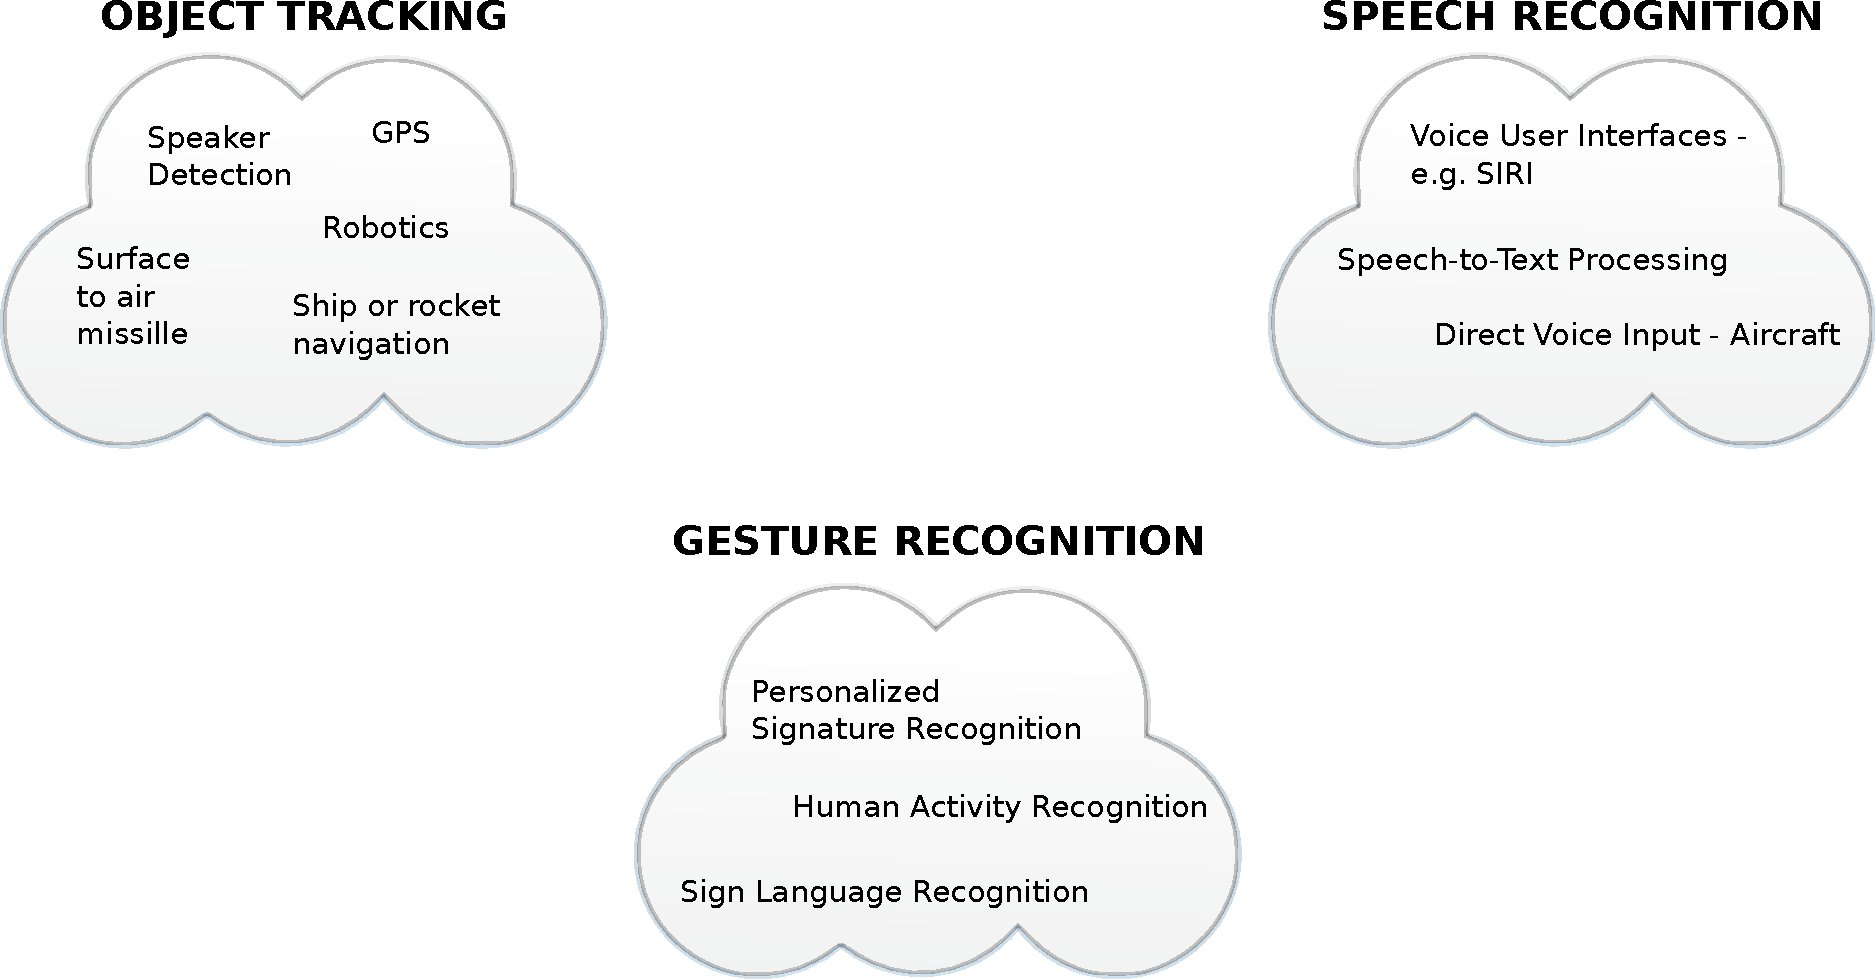
\includegraphics[width=\textwidth]{images/time_series_problems_1.pdf}
\end{frame}

\begin{frame}
  \frametitle{Sequence / Temporal problems (II)}
  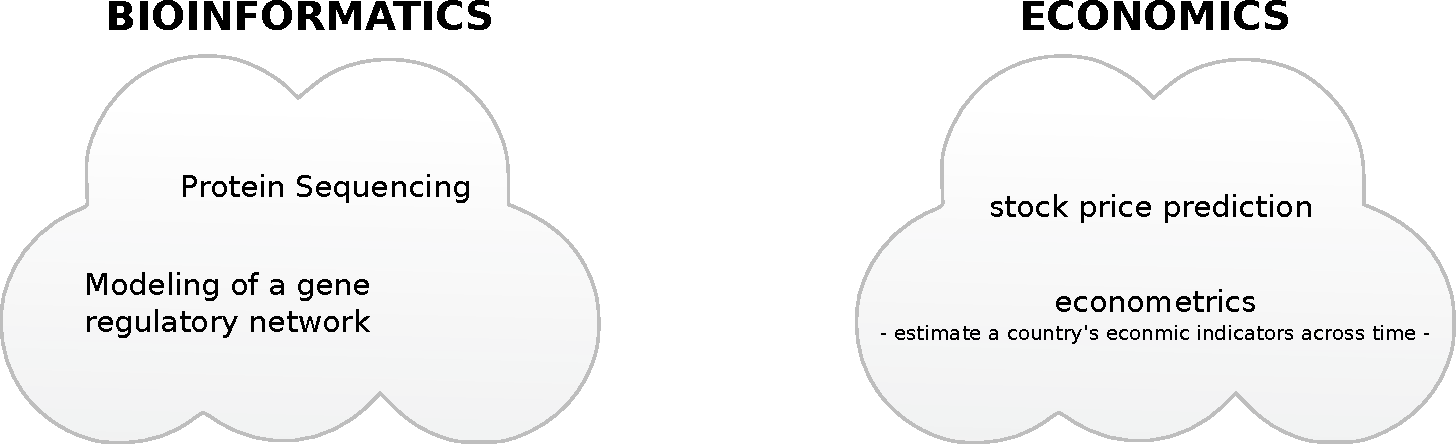
\includegraphics[width=\textwidth]{images/time_series_problems_2.pdf}
  %Koller and Frideman au scris in \cite{KollerFriedman09}
  % temporal sequences
  % DBN for ts
  % HMM as a special case of DBN
\end{frame}


% descrierea a ceea ce inseamna Probabilistic Reasoning over Time (capitol 15.2 AI a modern approach)
% 	- states and observations
\begin{frame}[t]
  \frametitle{Probabilistic Reasoning over Time - Models}
	Consider some of the previously presented problems ...
	\vspace*{0.5em}
	\pause	
	
	How do we model such dynamic situations? 
	\vspace*{1em}
	\pause	
	
	\textbf{States and Observations}
	\begin{itemize}
		\item The process of change is viewed as a series of \alert{time slices (snapshots)}
		\item Each time slice contains a set of random variables
    	\begin{itemize}
	    	\item $\mathbf{O}_t$ - set of all \alert{\emph{observable}} evidence variables at time \emph{t}
			\item $\mathbf{Q}_t$ - set of all \alert{\emph{unobservable / hidden}} state variables at time \emph{t}
		\end{itemize}
	\end{itemize}
\end{frame}

%	- stationary process, Markov assumption, Sensor model
\begin{frame}[t]
  \frametitle{Probabilistic Reasoning over Time - Assumptions}
	Consider some of the previously presented problems ...
	\vspace*{0.5em}
	\pause	
	
	What \alert{assumptions} (if any) do we make?
	\pause	
	
	\begin{block}{Stationary Process}
		The process of change is governed by laws \alert{that do not themselves change over time}.\\
		\alert{Implication:} we need to specify conditional distributions only for the variables within a \emph{representative} timeslice.
	\end{block}
	
	\pause	
	
	\begin{block}{Markov Assumption}
		The current state in a process of change depends only on a \alert{finite history} of previous states.
		\\
		\alert{Implication:} there is a \alert{bounded} number of ``parents'' for the variables in each time 
		slice.\\
		$\mathbf{P}(\mathbf{Q}_t \vert \mathbf{Q}_{1:t-1}) = \mathbf{P}(\mathbf{Q}_t \vert \mathbf{Q}_{t-1})$
		\hspace*{1em}
		$\mathbf{P}(\mathbf{O}_t \vert \mathbf{Q}_{1:t}, \mathbf{Q}_{1:t-1}) = \mathbf{P}(\mathbf{O}_t \vert \mathbf{Q}_t)$
	\end{block}
  
\end{frame}

%	- inference in temporal models
%		- filtering
%		- prediction
%		- smoothing (hindsight)
%		- most likely explanation
%		- model learning
\begin{frame}
  \frametitle{Probabilistic Reasoning over Time - Inference}
	What are the basic inference tasks that must be solved?
	\pause	
	
	\begin{block}{Filtering (monitoring)}
		The task of computing the \alert{belief state} - the posterior distribution over the 
		\alert{current state}, given all evidence to date.\\
		$\mathbf{P}(\mathbf{Q}_t \vert \mathbf{o}_{1:t})$
	\end{block}
	\pause
	
	\begin{block}{Evaluation (likelihood)}
		The task of computing the \alert{likelihood} of the evidence up to present.\\
		$\mathbf{P}(\mathbf{o}_{1:t})$
	\end{block}  
\end{frame}

\begin{frame}
  \frametitle{Probabilistic Reasoning over Time - Inference}
	\begin{block}{Prediction}
		The task of computing the posterior distribution over the \alert{future state}, 
		given all evidence to date.\\
		$\mathbf{P}(\mathbf{Q}_{t+k} \vert \mathbf{o}_{1:t})$, for some $k > 0$
	\end{block}
	\pause
	
	\begin{block}{Smoothing (hindsight)}
		The task of computing the posterior distribution over a \alert{past state}, 
		given all evidence to the present.\\
		$\mathbf{P}(\mathbf{Q}_k \vert \mathbf{o}_{1:t})$, for some $1 \le k < t$\\
		Provides a better estimate of the state than was available at the time.
	\end{block}
\end{frame}

\begin{frame}
  \frametitle{Probabilistic Reasoning over Time - Inference}
	\begin{block}{Most likely explanation}
		Given a \emph{sequence of observations}, find the \alert{sequence of states} that is 
		\alert{most likely} to have generated those observations.
		$argmax_{q_{1:t}}$ $\mathbf{P}(\mathbf{q}_{t+k} \vert \mathbf{o}_{1:t})$, for some $k > 0$
	\end{block}
	\pause
	
	\begin{block}{Learning}
		Given a set of \emph{observation sequences}, find a method to learn the \alert{transition} 
		(e.g. $P(q_{t+1} = s_j \vert q_t = s_i)$, $1 \le i,j < N$) and \alert{sensor} ($P(o_t \vert q_t)$) 
		\alert{models} from the observations.
	\end{block}
\end{frame}

\begin{frame}[t]
    \frametitle{Probabilistic Reasoning over Time - Known Methods}
    
  	\begin{block}{Dynamic Bayesian Networks (DBN)}
  		A DBN is Bayesian network that represents a temporal probability model.
  	\end{block}
  	
  	\begin{figure}
  		\centering
  		
		\begin{subfigure}[b]{0.18\textwidth}
			\centering
  			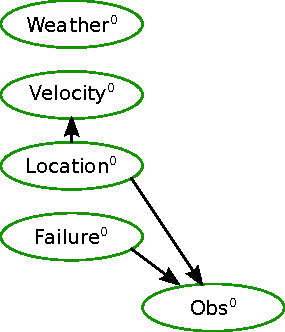
\includegraphics[width=\textwidth]{dbn-vehicle/zero.pdf}
  			\caption{\tiny{the 2-time-slice Bayesian Network}}
  			\label{fig:2TBN}
  		\end{subfigure}
  		\begin{subfigure}[b]{0.33\textwidth}
			\centering
			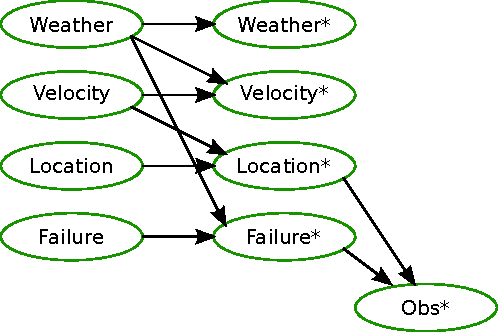
\includegraphics[width=\textwidth]{dbn-vehicle/transition.pdf}
  			\caption{\tiny{the time 0 network}}
  			\label{fig:zeroDBN}
  		\end{subfigure}
  		\begin{subfigure}[b]{0.39\textwidth}
			\centering
			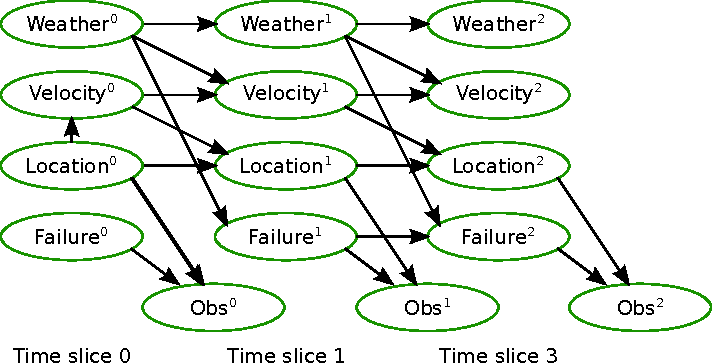
\includegraphics[width=\textwidth]{dbn-vehicle/unrolled.pdf} 
  			\caption{\tiny{unrolled DBN over 3 time slices}}
  			\label{fig:unrolledDBN}
  		\end{subfigure}
  		\caption{\tiny{A highly simplified DBN for monitoring a vehicle \parencite{KollerFriedman09}}}
  		\label{fig:DBN}
  	\end{figure}
  	
  	Applied in problems like: object tracking, human activity recognition, protein sequencing etc.
\end{frame}


\begin{frame}[t]
    \frametitle{Probabilistic Reasoning over Time - Known Methods}
  
  \begin{block}{Kalman Filters (Linear Dynamical Systems)}
  	A temporal model of one or more real-valued variables that \alert{evolve linearly} over time, with some 
  	\alert{Gaussian noise}.
  \end{block}
  
  \begin{columns}[T]
  	\column{0.4\textwidth}
  	\begin{figure}
  		\centering
  		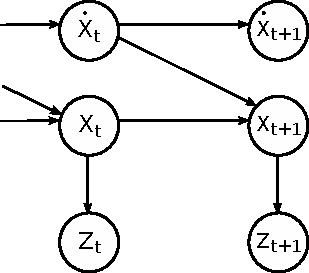
\includegraphics[height=0.35\textheight]{images/kalman_filter_simple.pdf}
  		\caption{\tiny{BN structure for a linear dynamical system with position $X_t$, 
  		velocity $\dot{X}_t$, and position measurement $Z_t$}}
  	\end{figure}
	  
  	\column{0.6\textwidth}
  	\begin{itemize}
  	\item \footnotesize{can be viewed as DBNs where all variables are continuous and all dependencies are 
  		linear gaussian}
  	\item \footnotesize{wide application in \textbf{object tracking}}
  \end{itemize}
  \end{columns}
  
\end{frame}

\begin{frame}[t]
    \frametitle{Probabilistic Reasoning over Time - Known Methods}
  
  \begin{block}{Hidden Markov Models (HMM)}
  	An HMM is a temporal probabilistic model in which the state of the process is described by 
  	\alert{a single discrete} random variable. The possible values of the variable are the possible states of the world.
  \end{block}
  
  \vspace*{1em}
  
  Used successfully in applications like:
  \begin{itemize}
  	\item Handwriting Recognition
  	\item Gesture Recognition
  	\item Speech Recognition
  	\item Part-of-Speech Tagging
  	\item DNA Sequencing
  \end{itemize}
\end{frame}


\section{Theory of HMMs}
\label{sec:theory}

\subsection{The 3 things you want from an HMM}
\label{sec:problems}

\begin{frame}
  
  The 3 fundamental problems \parencite{rabiner1989tutorial}
  \begin{itemize}
  	\item Particularization of temporal inference problems to the HMM case
  	\item The restricted structure of the HMM allows for elegant implementations of all the basic algorithms
  \end{itemize}
  \pause

  \begin{block}{Evaluation Problem}
    Given a model and a sequence of observations, how do we compute the probability that the \alert{observed 
    sequence} was produced by the model?
  \end{block}
  \pause
  \begin{block}{Best Explanation of Observations Problem}
    Given a model and a sequence of observations how do we choose a corresponding sequence of \alert{states} which 
    \emph{gives meaning} to the observations? How do we \emph{uncover} the hidden part of the model?
  \end{block}
  \pause
  \begin{block}{Model Estimation (Training) Problem}
    Given some observed sequences, how do we adjust the \alert{parameters} of an HMM model that best tries to explain 
    the observations? 
    
  \end{block}

\end{frame}


\subsection{Mathematical Foundations for HMMs}
\label{sec:math}



\begin{frame}
  \frametitle{An example problem: Emotional states}
  \begin{columns}[T]
    \column{0.58\textwidth}
    \only<1>{\framebox{
\includegraphics[width=\textwidth]{all/hmm-final-m.pdf}}}
    \only<2>{\framebox{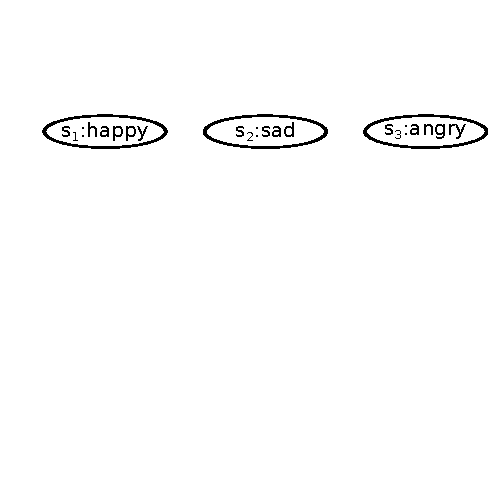
\includegraphics[width=\textwidth]{all/hmm-final-n.pdf}}}
    \only<3>{\framebox{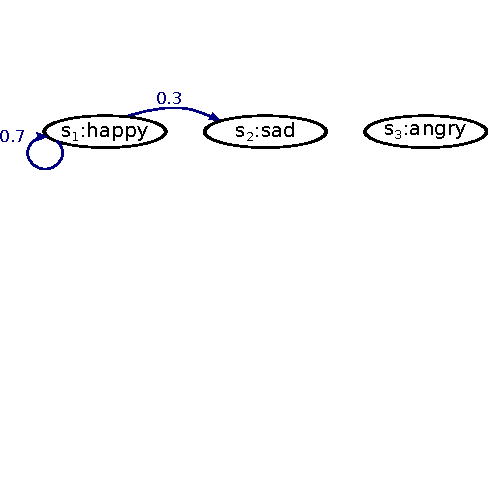
\includegraphics[width=\textwidth]{all/hmm-final-o.pdf}}}
    \only<4>{\framebox{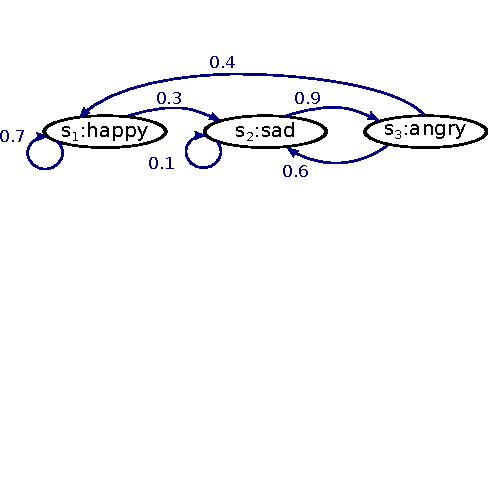
\includegraphics[width=\textwidth]{all/hmm-final-q.pdf}}}
    \only<5>{\framebox{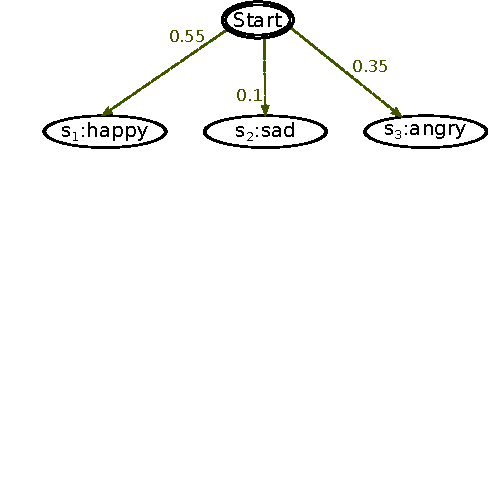
\includegraphics[width=\textwidth]{all/hmm-final-r.pdf}}}
    \only<6>{\framebox{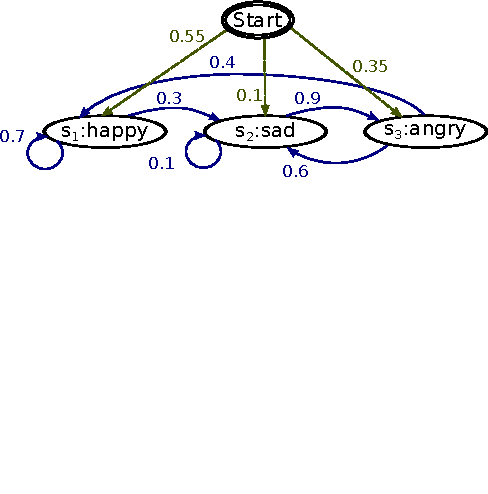
\includegraphics[width=\textwidth]{all/hmm-final-s.pdf}}}
    \only<7>{\framebox{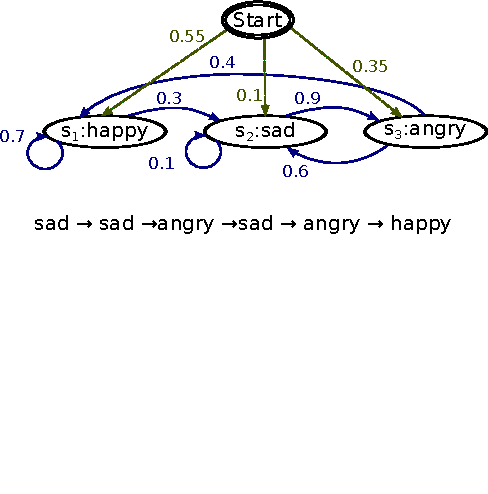
\includegraphics[width=\textwidth]{all/hmm-final-t.pdf}}}
    \only<8>{\framebox{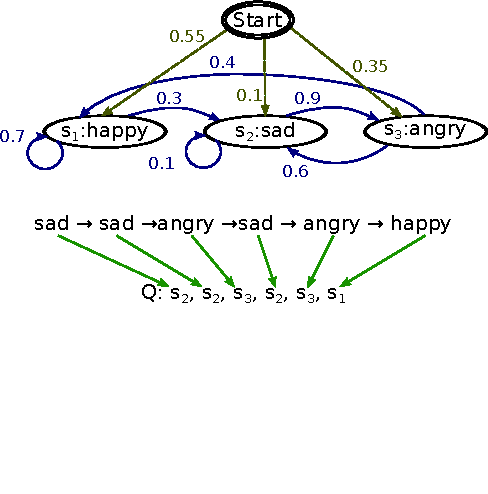
\includegraphics[width=\textwidth]{all/hmm-final-u.pdf}}}
    \only<9>{\framebox{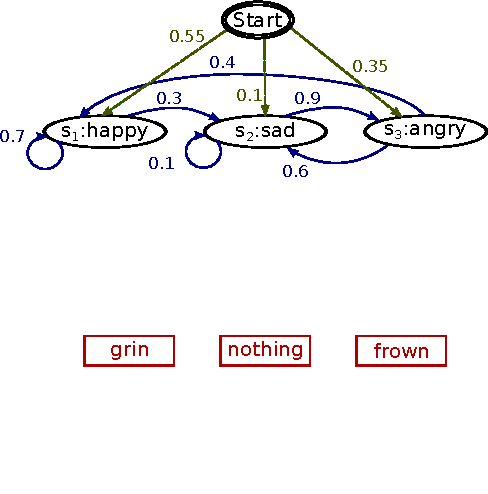
\includegraphics[width=\textwidth]{all/hmm-final-v.pdf}}}
    \only<10>{\framebox{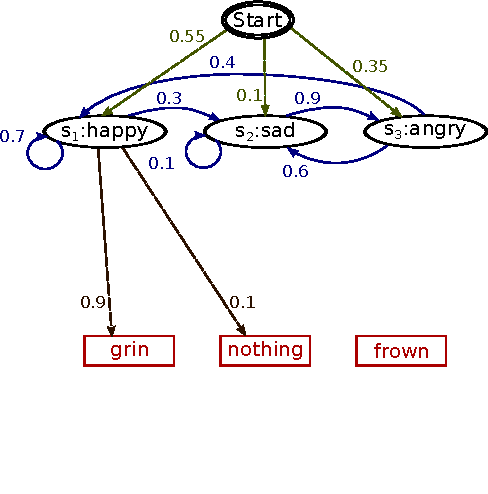
\includegraphics[width=\textwidth]{all/hmm-final-v2.pdf}}}
    \only<11-12>{\framebox{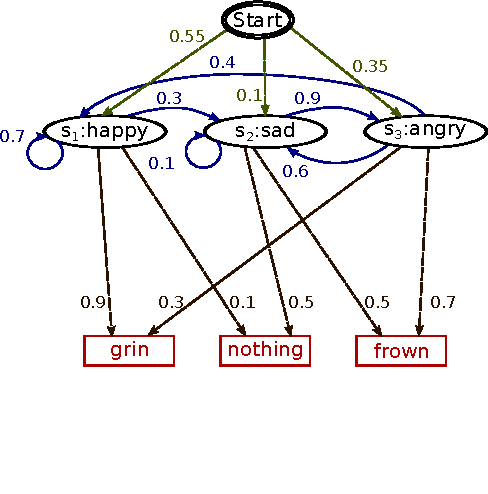
\includegraphics[width=\textwidth]{all/hmm-final-w.pdf}}}
    \only<13>{\framebox{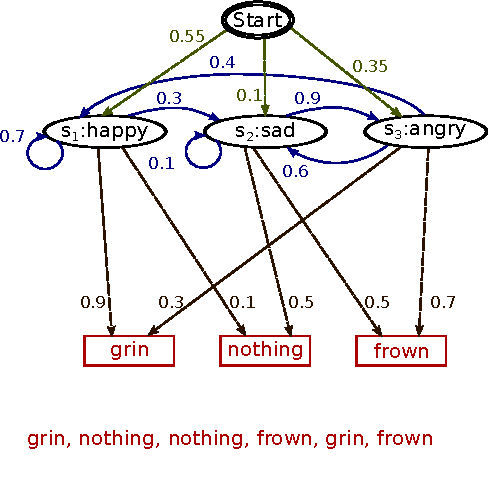
\includegraphics[width=\textwidth]{all/hmm-final-x.pdf}}}
    \only<14>{\framebox{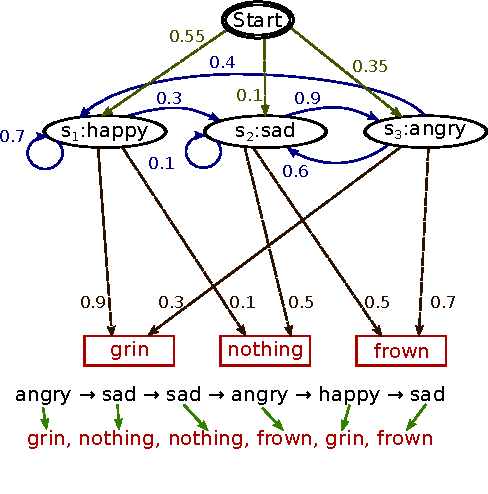
\includegraphics[width=\textwidth]{all/hmm-final-y.pdf}}}
    \only<15>{\framebox{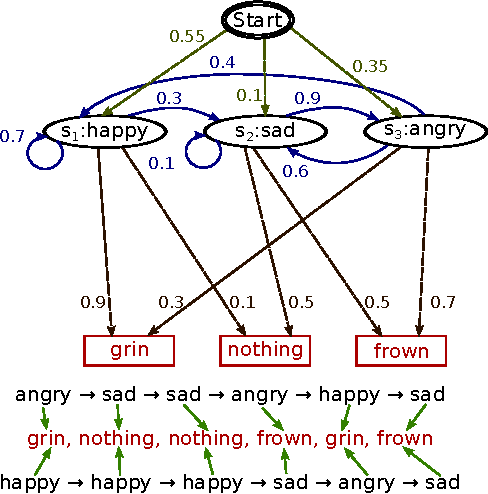
\includegraphics[width=\textwidth]{all/hmm-final-z.pdf}}}
    \only<16> {
      \begin{itemize}
      \item Example inspired from: \\\vspace*{1em}
        \fullcite{zubek2006introduction}
      \end{itemize}

    }
    

    \column{0.4\textwidth} \only<1>{ Let's consider a simple example:
      \\ \ a robot that tracks the emotional states of a player.  }
    \only<2>{ $\mathbf{N}$ - number of states \\ \vspace*{.5em}
      $\mathbf{N}=3$ \\ \vspace*{.5em} states:
      \begin{itemize}
      \item $s_1$: happy
      \item $s_2$: sad
      \item $s_3$: angry
      \end{itemize}

    }\only<3-4> { $\mathbf{A}$ - state transition probability
      distribution \\ \vspace*{.5em} \small{ $\mathbf{A} = \lbrace
        a_{i,j} \rbrace, \: 1 \le i, j \le N$ \\ \vspace*{.5em}
        $a_{i,j} = P(q_{t+1}=s_j \vert q_t = s_i)$
        \begin{itemize}
        \item $a_{\mathbf{1},1} = 0.7$
        \item $a_{\mathbf{1},2} = 0.3$
        \item $a_{\mathbf{1},3} = 0$
        \end{itemize}
        $\displaystyle\sum_{j=1}^{N}a_{i,j}=1, \quad 1 \le i \le N$ }
      \visible<4-> { $\mathbf{A} = \bordermatrix{~ & s_1 & s_2 & s_3
          \cr s_1 & 0.7 & 0.3 & 0 \cr s_2 & 0 & 0.9 & 0.1 \cr s_3 &
          0.4 & 0.6 & 0 \cr}$ }

    }
    
    \only<5>{ $\mathbf{\Pi}$ - initial state distribution \\
      \vspace*{0.5em} $\mathbf{\Pi} = \lbrace \pi_i \rbrace,\quad 1
      \le i \le N$ \\ \vspace*{0.5em} $\pi_i = P(q_1 = s_i)$ \\
      \vspace*{0.5em}
      
      $ \mathbf{\Pi} = \bordermatrix{ ~ & s_1 & s_2 & s_3 \cr ~ & 0.35
        & 0.1 & 0.55 \cr} $ }
    
    \only<6-8>{ $A = \bordermatrix{~ & s_1 & s_2 & s_3 \cr s_1 & 0.7 &
        0.3 & 0 \cr s_2 & 0 & 0.9 & 0.1 \cr s_3 & 0.4 & 0.6 & 0 \cr}$
      \\ \vspace*{0.25em} $\Pi = \bordermatrix{ ~ & s_1 & s_2 & s_3
        \cr ~ & 0.35 & 0.1 & 0.55 \cr}$ \\ \vspace*{0.25em}
      \visible<8> { $Q = [ q_1 q_2 \cdots q_T ]$ \small{
          \begin{equation*}
            \begin{split}
              P(Q & \vert A,\Pi)= \\ & = \pi_{q_1}a_{q_1,q_2}\cdots
              a_{q_{T-1},q_T}
            \end{split}
          \end{equation*}
          \begin{equation*}
            \begin{split}
              P(s_2,s_2,s_3,s_2,s_3,s_1\vert A,\Pi) = \\
              = \pi_2 \cdot a_{2,2} \cdot a_{2,3} \cdot a_{3,2} \cdot a_{2,3} \cdot a_{3,1} \\
              = \scriptstyle{0.1 \cdot 0.3 \cdot 0.1 \cdot 0.9 \cdot 0.6 \cdot 0.9 \cdot 0.4} \\
              = \scriptstyle{0.0005832}
            \end{split}
          \end{equation*}
        } }}

    \only<9>{ $\mathbf{M}$ - number of distinct observable values \\
      \vspace*{.5em} $\mathbf{M}=3$ \\ \vspace*{.5em} values:
      \begin{itemize}
      \item $v_1$: grin
      \item $v_2$: nothing
      \item $v_3$: frown
      \end{itemize}
    }

    \only<10-11> { $\mathbf{B}$ - observation values probability
      distribution \\ \vspace*{.5em} \small{ $\mathbf{B} = \lbrace
        b_{j,k} \rbrace \: \scriptstyle{1 \le j \le N, 1 \le k, \le
          M}$
        \begin{equation*}
          \begin{split}
            b_{j,k} & =b_{j}(v_k) \\
            & =P(o_t = v_k \vert q_t = s_j)
          \end{split}
        \end{equation*}
        \vspace*{-1.5em} \scriptsize{
          \begin{itemize}
          \item $b_{\mathbf{1},1} = b_{\mathbf{1}}(grin) = 0.9$
          \item $b_{\mathbf{1},2} = b_{\mathbf{1}}(nothing) = 0.1$
          \item $b_{\mathbf{1},3} = b_{\mathbf{1}}(frown) = 0$
          \end{itemize}}
        $\displaystyle\sum_{k=1}^{M}b_{j,k}=1, \quad 1 \le j \le N$\\
      }\visible<11> { $\mathbf{B} = \bordermatrix{ ~ & grin & notg &
          frown \cr s_1 & 0.9 & 0.1 & 0 \cr s_2 & 0 & 0.5 & 0.5 \cr
          s_3 & 0.3 & 0 & 0.7 \cr }$ } }
    
    \only<12>{ $\mathbf{\lambda}$ - parameters of the model \\
      \vspace*{.5em} $\lambda = (A, B, \Pi)$ \\ \vspace*{2em} $A$ -
      state transition probability distribution \\ \vspace*{.5em} $B$
      - observation values probability distribution \\ \vspace*{.5em}
      $\Pi$ - initial state distribution }
    
    \only<13-15>{ $\mathbf{O}$ - observation sequence \\ \vspace*{1em}
      $\mathbf{T}$ - length of observation sequence \\ \vspace*{1em}
      $O = [ o_1 o_2 \cdots o_T ]$ }

    
  \end{columns}
\end{frame}


\begin{frame}
  \frametitle{Restating the three fundamental HMM Problems}
  \begin{block}{Evaluation Problem}
    Given a model and a sequence of observations, how do we compute
    the probability that the \alert{observed sequence} was produced by
    the model?
  \end{block}
  \pause
  \begin{equation}
    P(O \vert Q, \lambda) = \displaystyle\prod_{t=1}^{T} P(o_t \vert
    q_t, \lambda)= \displaystyle\prod_{t=1}^{T} b_{q_t}(o_t) =
    b_{q_1}(o_1) \cdot \ldots \cdot b_{q_T}(o_T)
    \label{eq:pql}
  \end{equation}\pause
  \begin{equation}
    P(Q | \lambda) = \pi_{q_1}\displaystyle\prod_{t=2}^{T}
    a_{q_{t-1},q_t} = \pi_{q_1} \cdot a_{q_1,q_2} \cdot a_{q_2,q_3} \cdot \ldots \cdot
    a_{q_{T-1},q_T}\label{eq:pql2}
  \end{equation}\pause
  \begin{equation}
    \begin{split}
      P(O \vert \lambda) = \displaystyle\sum_{all\;Q} P(O, Q \vert
      \lambda) & = \displaystyle\sum_{all\;Q} P(O,\vert Q, \lambda)
      \cdot P(Q, \lambda) \\
      & = \displaystyle\sum_{all\;Q} \Big( \pi_{q_1} \cdot
      b_{q_1}(o_1) \cdot \displaystyle\prod_{t=2}^{T} b_{q_t}(o_t)
      a_{q_{t-1},q_t} \Big)
    \end{split}
    \label{eq:pql3}
  \end{equation}
\end{frame}


\subsection{Notation Conventions \& Framework Description}
\label{sec:octave}

\begin{frame}
  \frametitle{Notation Conventions}

  
\end{frame}


\begin{frame}
  \frametitle{Variables in Octave}

  
\end{frame}

\section{Implementing HMMs}
\label{sec:implementation}

\subsection[Forward-Backward algorithm]{Using the Model for
  Estimations: the Forward-Backward algorithm}
\label{sec:fb}

\begin{frame}
  \frametitle{$\alpha$ (forward) variables}
  \begin{itemize}
  \item Can we \emph{efficiently} compute $P(O \vert \lambda)$?\\
    \vspace*{.5em} Yes, using the \textbf{forward-backward} algorithm
    \vspace*{1em} \pause
  \item Introducing $\alpha$ (forward) variables:
    \begin{equation}
      \label{eq:alpha}
      \begin{split}
        \alpha_{t,i}=P(o_1,o_2,\ldots,o_t, q_t = S_i \vert \lambda) \\
        \scriptstyle{1 \le t \le T, 1 \le i \le N}
      \end{split}
    \end{equation}
    \pause
  \item Relation between $P(O \vert \lambda)$ and $\alpha$ variables:
    \begin{equation}
      \label{eq:eq1toalpha}
      P(O \vert \lambda) = \displaystyle\sum_{i=1}^{N}\alpha_{T,i}
    \end{equation}
  \end{itemize}
\end{frame}


\begin{frame}
  \frametitle{Computing $\alpha$ variables}
  \begin{columns}
    \column{0.38\textwidth}
    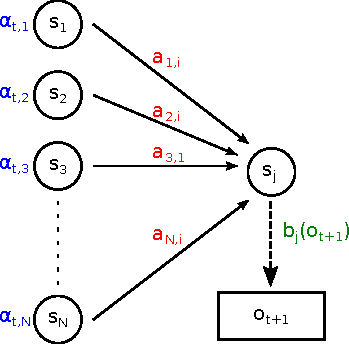
\includegraphics[width=\textwidth]{graphics/forward.pdf}
    \column{0.62\textwidth}
    \begin{itemize}
    \item $\alpha$ variables initialization \\
      $P(o_1,q_1=s_i) = P(o_1 \vert q_1=s_i)P(q_1=s_i)$ \\
      $\alpha_{1,i}=\pi_ib_i(o_1), \quad 1 \le i \le N$ \pause
    \item Induction step
      \begin{equation*}
        \label{eq:alpha_induct}
        \alpha_{t+1,j}=\Big[ \displaystyle\sum_{i=1}^{N}\alpha_{t,j}a_{i,j}\Big] b_{j}(o_{t+1}), \quad \substack{1 \le t \le T-1, \\ 1 \le j \le N}
      \end{equation*}
    \item Probability of the observed sequence
      \begin{equation*}
        \label{eq:alpha_term}
        P(O \vert \lambda) = \displaystyle\sum_{i=1}^{N}\alpha_{T,i}
      \end{equation*}
    \end{itemize}
  \end{columns}
\end{frame}

\begin{frame}
  \frametitle{$\beta$ (backward) variables}
  \begin{itemize}
  \item Introducing $\beta$ (backward) variables:
    \begin{equation}
      \label{eq:beta}
      \beta_{t,i}=P(o_{t+1} o_{t+2} \cdots o_{T} \vert q_t = S_i, \lambda)
    \end{equation}
    \vspace*{1em} \pause
  \item $\beta$ variables are not needed to compute $P(O \vert
    \lambda)$, but they are useful for the other two problems
  \item $\beta$ variables can be computed in a similar (efficient) way
    to the procedure for the $\alpha$ variables
  \end{itemize}
\end{frame}

\begin{frame}
  \frametitle{Computing $\beta$ variables}
  \begin{columns}[B]
    \column{0.55\textwidth}
    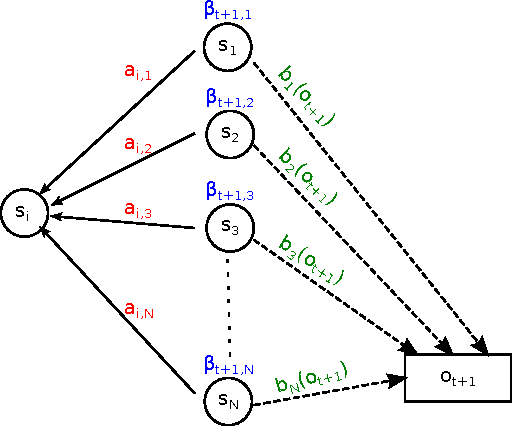
\includegraphics[width=\textwidth]{graphics/backward.pdf}
    \column{0.4\textwidth}
    \begin{itemize}
    \item $\beta$ variables initialization \\
      $\beta_{T,i}=1,\quad 1 \le i \le N$
    \end{itemize}
  \end{columns}
  \begin{itemize}
  \item Induction step \\
    $\beta_{t,i}=\displaystyle\sum_{j=1}^{N}a_{i,j}b_j(o_{t+1})\beta_{t+1,j},
    \quad t = T-1, T-2, \ldots , 1, 1 \le i \le N$
  \end{itemize}
\end{frame}

\begin{frame}
  \frametitle{Scaling problems}
  \begin{itemize}
  \item Remember $P(O \vert \lambda)$:
    \begin{equation*}
      P(O \vert \lambda) =  \displaystyle\sum_{\text{all}\;Q} \Big( \pi_{q_1} \cdot
      b_{q_1}(o_1) \cdot \displaystyle\prod_{t=2}^{T} b_{q_t}(o_t)
      a_{q_{t-1},q_t} \Big)
    \end{equation*}
    \pause
  \item for large sequences, terms are very close to zero and exceed
    precision range
  \item a scaling mechanism is needed
  \end{itemize}
\end{frame}

\begin{frame}
  \frametitle{The Forward-Backward algorithm with scaling}
  \begin{itemize}
  \item $\hat{\alpha}_{t,i}$ - scaled $\alpha$ variables
  \item $\hat{\beta}_{t,i}$ - scaled $\beta$ variables \vspace*{1em}
  \item $C_t$ - scaling coefficients \vspace*{1em}
  \item Scaled $\alpha$ variables
    \begin{equation}
      \label{eq:scaled-alpha}
      \bar{\alpha}_{t,i} = C_t \cdot \alpha_{t,i}
    \end{equation}
  \item Scaled $\beta$ variables
    
    \begin{equation}
      \label{eq:scaled-beta}
      \bar{\beta}_{t,j} = C_t \cdot \beta_{t,j}
    \end{equation}
  \end{itemize}
\end{frame}

\begin{frame}
  \frametitle{Computing scaled values}
  \begin{itemize}
  \item \emph{Scaled} intialization:
    \begin{align}
      \ddot{\alpha}_{1,i} = \alpha_{1,i},\quad 1 \le i \le N \\
      c_1 = \frac{1}{\displaystyle\sum_{i=1}^{N} \ddot{\alpha}_{1,i}} \\
      \hat{\alpha}_{1,i} = c_1 \cdot \ddot{\alpha}_{1,i}, \quad 1 \le
      i \le N
    \end{align}
    \pause
    \vspace*{-.5em}
  \item \emph{Scaled} induction step:
    \begin{align}
      \ddot{\alpha}_{t+1,i} = \Big[
      \displaystyle\sum_{i=1}^{N}\hat{\alpha}_{t,i}a_{i,j}\Big]
      b_{j}(o_{t+1}) \\
      c_{t+1} = \frac{1}{\displaystyle\sum_{i=1}^{N} \ddot{\alpha}_{t+1,i}} \\
      \hat{\alpha}_{t+1,i} = c_{t+1} \cdot \ddot{\alpha}_{t+1,i},
      \quad 1 \le i \le N
    \end{align}
  \end{itemize}

\end{frame}

\begin{frame}
  \frametitle{Computing $P(O | \lambda)$}
  \begin{equation}
    \label{eq:scaled-probability}
    P(O \vert \lambda) = \frac{1}{C_T}
  \end{equation}
\end{frame}


\begin{frame}
  \frametitle{Let's write some code}
  \begin{itemize}
  \item You will implement now the forward-backward algorithm in
    Octave
  \item Write code to compute:
    \begin{itemize}
    \item the
    \end{itemize}

  \end{itemize}
\end{frame}

\subsection[Baum-Welch algorithm]{Learning from Observations:
  Baum-Welch algorithm}
\label{sec:bw}

\begin{frame}[t]
	\frametitle{Learning from observations - Reminder}
	\begin{block}{Model Estimation (Training) Problem}
    	Given some observed sequences, how do we adjust the \alert{parameters} of an HMM model that best tries 	
    	to explain the observations?
  	\end{block}
  	\pause
  	
  	\begin{block}{}
  		Adjust the model parameters $\lambda = (A, B, \Pi)$ to obtain $\max_{\lambda} P(O \vert \lambda)$
  	\end{block}
  	\pause
  	
  	\begin{block}{}
  		The observation sequence used to adjust the model parameters is called a \alert{training} sequence.\\
  		Training problem is crucial - allows to create best models for real phenomena.
  	\end{block}
\end{frame}


\begin{frame}[t]
	\frametitle{Learning from observations - Aspects of the approach}
	\pause
		
	\begin{block}{\alert{Problem}}
    	There is no known way to analytically solve for the model which maximizes the probability of the
    	observation sequence.
  	\end{block}
  	\pause
  	
  	\begin{block}{Solution}
  		We can choose $\lambda = (A, B, \Pi)$ such that $\max_{\lambda} P(O \vert \lambda)$ is 
  		\alert{locally maximized} using an \alert{iterative procedure} such as \emph{Baum-Welch}.\\
  		The method is an instance of the \emph{EM algoritm} \parencite{dempster1977maximum} for HMMs.
  	\end{block}
  	
\end{frame}

\begin{frame}[t]
	\frametitle{Baum-Welch algorithm (I)}
	\pause
	We first define some auxiliary variables:
	
	\begin{block}{}    
    	$\xi_{t,i,j} = \xi_t(i,j) = P(q_t=s_i,q_{t+1}=s_j \vert O, \lambda)$\\
    	The probability of being in state $s_i$ at time $t$ and in state $s_j$ at time $t+1$, given
    	the model and the observation sequence.
	\end{block}
	\pause
	
	\begin{block}{}    
    	$ \gamma_{t,i} = \gamma_t(i) = P(q_t = s_i \vert O, \lambda)$\\
    	The probability of being in state $s_i$ at time $t$, given the model and the observation sequence.
	\end{block}
	\vspace*{1em}
	\pause
	
	From the definitions it follows that:\\
	$ \gamma_t(i) = \displaystyle\sum_{j=1}^{N}\xi_t(i,j)$
  	
\end{frame}

\begin{frame}[t]
	\frametitle{Baum-Welch algorithm (II)}
	\begin{columns}[T]
	
	\column{0.42\textwidth}
	\begin{figure}
  		\centering
		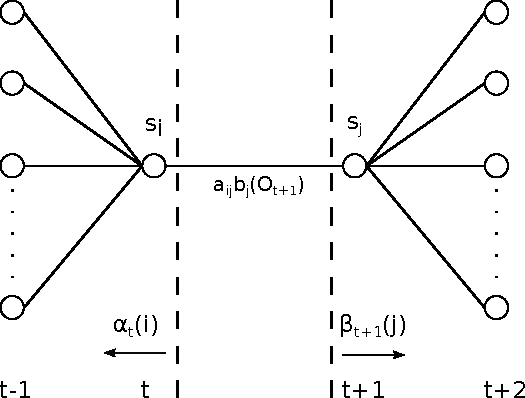
\includegraphics[height=0.40\textheight]{images/baum-welch-alg.pdf}
		\caption{\tiny{Sequence of operations required for the computation of the joint event that the system 
		is in state $S_i$ at time $t$ and state $S_j$ at time $t+1$} \parencite{rabiner1989tutorial}}
		\label{fig:baum-welch-alg}
  	\end{figure}	
	
	\column{0.58\textwidth}
		\begin{equation*}		
		\alpha_{t,i}=P(o_1,o_2,\ldots,o_t, q_t = S_i \vert \lambda)
		\end{equation*}
		
		\begin{equation*}
		\beta_{t,i}=P(o_{t+1} o_{t+2} \cdots o_{T} \vert q_t = S_i, \lambda)
		\end{equation*}
		\footnotesize
		
		\begin{equation*}
			\begin{split}
		      \xi_t(i,j) & = \frac{\alpha_{t,i}\cdot a_{i,j} \cdot
		        b_j(o_{t+1}) \cdot \beta_{t+1,j}}
		      {P(O \vert \lambda)} \\
		      & = \frac{\alpha_{t,i}\cdot a_{i,j} \cdot b_j(o_{t+1}) \cdot
		        \beta_{t+1,j}}{
		        \displaystyle\sum_{k=1}^{N}\displaystyle\sum_{l=1}^{N}
		        \alpha_{t,k}\cdot a_{k,l} \cdot b_l(o_{t+1}) \cdot
		        \beta_{t+1,l}}
		    \end{split}
		\end{equation*}	
		\normalsize
	\end{columns}
	
\end{frame}

\begin{frame}
	\frametitle{Baum-Welch algorithm (III)}
	How do these auxiliary variables help?
	\vspace*{1em}
	
	\begin{block}{}
	$\displaystyle\sum_{t=1}^{T-1}\gamma_t(i)$ = expected number of transitions from $S_i$
	\end{block}
	\vspace*{1em}
	\begin{block}{}
	$\displaystyle\sum_{t=1}^{T-1}\xi_t(i,j)$ = expected number of transitions from $S_i$ to $S_j$
	\end{block}
	
\end{frame}

\begin{frame}[t]
	\frametitle{Baum-Welch algorithm (IV)}
	\footnotesize
	\begin{equation*}
	\bar{\pi_i} = \mbox{ expected no. of times in state } S_i \mbox{ at time } (t=1) = \gamma_t(i)
	\end{equation*}
	\pause	
	
	\begin{equation*}
	\begin{split}
	\bar{a_{i,j}} & = \frac{\mbox{expected no. of transitions from } S_i \mbox{ to } S_j}
							{\mbox{expcted no. of transition from } S_i} \\
				  & = \frac{\displaystyle\sum_{t=1}^{T-1}\xi_t(i,j)}
				   			{\displaystyle\sum_{t=1}^{T-1}\gamma_t(i)}	
	\end{split}
	\end{equation*}
	\pause	
	
	\begin{equation*}
	\begin{split}
	\bar{b_{j,k}}  & = \frac{\mbox{expected no. of times in } S_j \mbox{ observing symbol } v_k}
							{\mbox{expcted no. of times in } S_j} \\
				   & = \frac{\displaystyle\sum_{t=1, O_t = v_k}^{T}\gamma_t(j)}
				   			{\displaystyle\sum_{t=1}^{T}\gamma_t(j)}	
	\end{split}
	\end{equation*}	
	\normalsize	
\end{frame}

\begin{frame}[fragile, t]
	\frametitle{Baum-Welch algorithm (V)}
	The routine for the general case:
	\vspace*{1em}
	\lstset{columns=fullflexible, 
			basicstyle=\footnotesize, 
			numbers=left, 
			stepnumber=1, 
			numbersep=5pt,
			title=Baum-Welch Iterative Update,
			frame=single,
			xleftmargin=1em,
			captionpos=b}	

	\begin{lstlisting}[mathescape]
    Initialize uniform $\pi_i$ for $1 \le i \le N$
    Initialize random (stochastic) $a_{i,j}$
    Initialize uniform $b_{j,k}$ for $1 \le k \le M$
	
    Repeat until convergence
        E step:
            compute auxiliary variables $\xi_t(i,j)$ and $\gamma_t(i)$ 
            using current $\pi_i$, $a_{i,j}$ and $b_{j,k}$
        
        M step:
            compute updated parameter models $\bar{\pi_i}$, $\bar{a_{i,j}}$, $\bar{b_{j,k}}$
	\end{lstlisting}

\end{frame}

\begin{frame}
	\frametitle{Baum-Welch - Let's write some code}
	\centering
	LET'S WRITE SOME CODE :-)
\end{frame}
%% Tudor Berariu, Alexandru Sorici
%% Noiembrie 2012


\begin{frame}
  \frametitle{Problema interpretării}
  \begin{block}{Problema interpretării unei secvențe de observații}
    Date fiind un model   \alert{$\lambda=(A,B,\Pi)$} și o
    secvență de observații \alert{$O = [ o_1 o_2 \cdots o_T ]$}, 
    cum alegem o secvență corespunzătoare de stări
    \alert{$Q_{\text{best}} = [ q_{1_{\text{best}}} q_{2_{\text{best}}} \cdots q_{T_{\text{best}}} ]$} care \emph{să
      dea un înțeles} observațiilor? Cum \emph{descoperim} partea
    ascunsă a modelului?
  \end{block}\pause
  \begin{itemize}
  \item Răspunsul depinde de criteriul cu care alegem \emph{cea mai bună} secvență\pause
    \begin{itemize}
    \item \alert{secvența celor mai probabile stări $q_{t_{\text{best}}}$} (luate individual), date fiind modelul și secvența observată:\\
      $q_{t_{\text{best}}} = \underset{s_i}{\operatorname{argmax}}\; P(q_t = s_i \vert O, \lambda)$
    \item \alert{cea mai probabilă secvență de stări $Q$} (per ansamblu), date fiind modelul și secvența observată:\\
      $Q_{\text{best}} = \underset{\text{all }Q}{\operatorname{argmax}}\; P(Q \vert O, \lambda)$
    \end{itemize}
  \end{itemize}
\end{frame}


\begin{frame}
  \frametitle{Secvența celor mai probabile stări}
  Notație: $P(q_t = s_i \vert O, \lambda) = \mathbf{\gamma_{t,i}} = 
  \frac{\alpha_{t,i}\beta_{t,i}}{\displaystyle\sum_{j=1}^{N}\alpha_{t,j}\beta_{t,j}}$
  \begin{itemize}
  \item Este un criteriu satisfăcător?\pause
  \item \textbf{NU!}\\Pot exista $q_t$ și $q_{t+1}$ astfel încât $a_{q_t,q_{t+1}}=0$
  \end{itemize}
    % \begin{itemize}      
  % \item How can we answer the \emph{best explanation} problem?  \pause
  % \item \textbf{Individually} most likely states
  %   \begin{equation}
  %     \label{eq:individually}
  %     \gamma_{t,i}=P(q_t = s_i \vert O, \lambda)
  %   \end{equation}
  %   \pause
  % \item Computation
  %   \begin{equation}
  %     \label{eq:gamma_formula}
  %     \gamma_{t,i}=\frac{\alpha_{t,i}\beta_{t,i}}{P(O\vert \lambda)} =
  %     \frac{\alpha_{t,i}\beta_{t,i}}{\displaystyle\sum_{k=1}^{N}\alpha_{t,k}\beta_{t,k}}
  %   \end{equation}
  %   \pause
  % \item Problems?
  % \end{itemize}

\end{frame}

\begin{frame}
  \frametitle{Algoritmul Viterbi}
  \begin{itemize}
  \item Criteriu care ia în considerare distribuțiile de probabilitate 
    ale tranzițiilor între stări
  \item Cea mai bună cale:
    $Q_{\text{best}} = [q_{1_{\text{best}}} q_{2_{\text{best}}} \cdots q_{T_{\text{best}}}]$
    \begin{equation}
      Q_{\text{best}} = \underset{Q}{\operatorname{argmax}}\;
      P(Q \vert O, \lambda)
      = \underset{Q}{\operatorname{argmax}}\; P(Q, O \vert \lambda)
      \tag{\ref{eq:best-explanation}}
    \end{equation}
  \item \textbf{Algoritmul Viterbi} - programare dinamică
  \item Vom introduce variabilele $delta$.
  \end{itemize}
\end{frame}

\begin{frame}
  \frametitle{Variabilele $\delta$ - intuiție}
  \begin{block}{Întrebare}
    Dacă $Q = [q_1, q_2, \ldots, q_{t-1}, q_{t}]$ este cea mai bună secvență care explică $O = [o_1, o_2, \ldots o_{t-1}, o_{t}]$, atunci putem afirma că $Q[1:t-1]$ este cea mai bună secvență de stări care explică $O[1:t-1]$?
  \end{block}
  \pause
  \vspace*{1em}
  \begin{itemize}
  \item \textbf{NU!}
    \begin{align*}
        & P(q_1 = s_{i_1}, q_2 = s_{i_2}, \ldots, q_{t-1} = s_{i_{t-1}}, q_{t} = s_{i_{t}}\vert O, \lambda) = \\
        & P(q_1, q_2, \ldots, q_{t-1} \vert O, \lambda) \cdot  P(q_t = s_{i_t} \vert q_{t-1}= s_{i_{t-1}}, \lambda) \cdot P(o_t \vert q_t=s_{i_t}, \lambda)
      \end{align*}
    \end{itemize}
\end{frame}

\begin{frame}
  \frametitle{Variabilele $\delta$}
  \begin{itemize}
  \item Vom numi variabile $\delta$:
    \begin{equation}
      \label{eq:delta-definition}
      \delta_{t,i}=\underset{q_1,\ldots,q_{t-1}}{\operatorname{max}}
      P([q_1 q_2 \ldots q_{t-1} s_i], [o_1, o_2, \ldots o_t] \vert \lambda)
    \end{equation}
  \end{itemize}
  \begin{columns}
    \column{0.45\textwidth}
    \begin{itemize}
    \item $\mathbf{\delta_{t,i}}$ - cea mai mare probabilitate a unei secvențe de 
      stări de lungime $t$ care ajunge în $s_i$ și explică primele $t$ valori observate
      \visible<2>{
      \item relația dintre variabilele $\delta$:
        \begin{equation}
          \label{eq:delta-recurrence}
          \delta_{t+1,j} = [\underset{i}{\operatorname{max}}\; 
          \delta_{t,i} \cdot a_{i,j}] \cdot b_{j}(o_{t+1})
        \end{equation}}
    \end{itemize}
    \column{0.45\textwidth} \visible<2>{
      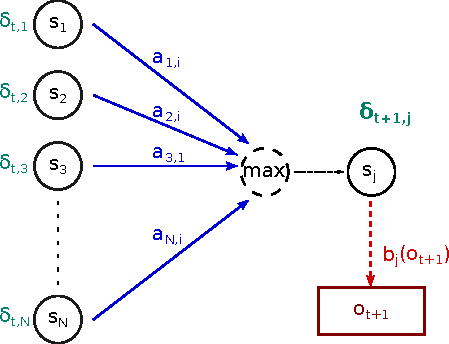
\includegraphics[width=\textwidth]{graphics/viterbi/general/viterbi-path.pdf}
    }
  \end{columns}
\end{frame}

\begin{frame}
  \frametitle{Algoritmul Viterbi - Privire de ansamblu}
  \begin{block}{Pași înainte}
    Calculăm cea mai mare probabilitate de a ajunge în starea $s_i$ 
    la momentul $t$ pe baza celor mai mari probabilități de a fi ajuns în 
    toate stările $s_j$ la $t-1$.
  \end{block}
  \pause
  \begin{block}{La final ($t=T$)}
    Starea finală este acea stare $s_i$ cu cea mai mare probabilitate de a ajunge
    la ea după observarea tuturor valorilor.
  \end{block}
  \pause
  \begin{block}{Pași înapoi}
    Refacem \emph{cea mai bună cale} alegând pentru fiecare moment $t$ starea care a
    dus la probabilitatea maximă pentru starea de la $t+1$.
  \end{block}
\end{frame}

\begin{frame}
  \frametitle{Algoritmul Viterbi (I)}
  \begin{description}
  \item[1] Inițializare: \\
    \begin{equation}
      \label{eq:viterbi-initialization}
      \begin{split}
        \delta_{1,i} & = \pi_{i}b_i(o_1), \quad 1 \le i \le N \\
        \psi_{1,i} & = 0
      \end{split}
    \end{equation}
  \item[2] Recursivitate: \\
    \begin{equation}
      \label{eq:viterbi-recursion}
      \begin{split}
        \delta_{t,j} & = [\underset{i }{\operatorname{max}}\; \delta_{t-1,i} \cdot
        a_{i,j}] \cdot b_{j}(o_{t})
        \quad \scriptstyle{2 \le t \le T, 1 \le j \le N} \\
        \psi_{t,i} & = \underset{i}{\operatorname{argmax}}\; \delta_{t-1,i}\cdot
        a_{i,j} \quad \scriptstyle{2 \le t \le T, 1 \le j \le N}
      \end{split}
    \end{equation}
  \end{description}
\end{frame}

\begin{frame}
  \frametitle{Algoritmul Viterbi (II)}
  \begin{description}
  \item[3] Terminare: \\
    \begin{equation}
      \label{eq:viterbi-termination}
      \begin{split}
        P(Q_{\text{best}} \vert O, \lambda) & = \underset{i}{\operatorname{max}}\; \delta_{T,i} \\
        q_{T_{\text{best}}} & = \underset{i}{\operatorname{argmax}}\; \delta_{T,i}
      \end{split}
    \end{equation}
  \item[4] Backtracking: \\
    \begin{equation}
      \label{eq:viterbi-backtracking}
      q_{t_{\text{best}}} = \psi_{t+1}(q_{t+1_{\text{best}}}), \quad \scriptstyle{t=T-1,T-2,\cdots, 1}
    \end{equation}
  \end{description}
\end{frame}

\begin{frame}
  \frametitle{Probleme numerice}
  \begin{itemize}
  \item Cine este $P(Q_{\text{best}} \vert O, \lambda)$?
    \begin{equation*}
      \begin{split}
        P(Q_{\text{best}} \vert O, \lambda) & = \delta_{T,i_T} \\
        P(Q_{\text{best}} \vert O, \lambda) & = \delta_{T-1,i_{T-1}} \cdot a_{i_{T-1},i_T} 
        \cdot b_{T}(o_{T})\\
        P(Q_{\text{best}} \vert O, \lambda) & = \delta_{T-2,i_{T-2}} \cdot a_{i_{T-2},i_{T-1}}
        \cdot b_{T-1}(o_{T-1}) \cdot a_{i_{T-1},j_T} \cdot b_{T}(o_{T})\\
        P(Q_{\text{best}} \vert O, \lambda) & = \displaystyle\prod \ldots
      \end{split}
    \end{equation*}
  \item Cum putem evita apropierea rapidă de zero?\pause
  \item Calculăm \alert{$log(P)$}
    \begin{equation*}
      \begin{split}
        \log(P(Q_{\text{best}} \vert O, \lambda)) & = \log(\delta_{T,i_T}) \\
        \log(P(Q_{\text{best}} \vert O, \lambda)) & = \log(\delta_{T-1,i_{T-1}}) + \log(a_{i_{T-1},i_T})
        + \log(b_{T}(o_{T}))\\
        \log(P(Q_{\text{best}} \vert O, \lambda)) & = \log(\delta_{T-2,i_{T-2}}) + \log(a_{i_{T-2},i_{T-1}})
        +\log(b_{T-1}(o_{T-1})+\log(a_{i_{T-1},j_T})+\log(b_{T}(o_{T}))\\
        \log(P(Q_{\text{best}} \vert O, \lambda)) & = \displaystyle\sum \ldots
      \end{split}
    \end{equation*}
    
  \end{itemize}
\end{frame}

\begin{frame}
  \frametitle{Probleme numerice - Rezolvare}
  \begin{itemize}
  \item Notație:
    \begin{equation*}
      \phi_{t,i}=\underset{q_1,\ldots,q_{t-1}}{\operatorname{max}}
      \log(P(q_1,\ldots,q_{t-1},q_t=s_i,o_1,\ldots,o_t\vert \lambda))=\log(\delta_{t,i})
    \end{equation*}
  \item Matricele $\log(\Pi)$, $\log(A)$ și $\log(B)$ pot fi precalculate.
  \end{itemize}
\end{frame}

\begin{frame}
  \frametitle{Algoritmul Viterbi - $log(P)$ (I)}
  \begin{description}
  \item[1] Inițializare: \\
    \begin{equation}
      \label{eq:viterbi-initialization}
      \begin{split}
        \phi_{1,i} & = \log(\pi_{i}) \mathbf{+} \log(b_i(o_1)), \quad 1 \le i \le N \\
        \psi_{1,i} & = 0
      \end{split}
    \end{equation}
  \item[2] Recursivitate: \\
    \begin{equation}
      \label{eq:viterbi-recursion}
      \begin{split}
        \phi_{t,j} & = [\underset{i}{\operatorname{max}}\; \phi_{t-1,i} \mathbf{+}
        log(a_{i,j})] \mathbf{+} \log(b_{j}(o_{t}))
        \quad \scriptstyle{2 \le t \le T, 1 \le j \le N} \\
        \psi_{t,i} & = \underset{i}{\operatorname{argmax}}\; \phi_{t-1,i} \mathbf{+}
        \log(a_{i,j}) \quad \scriptstyle{2 \le t \le T, 1 \le j \le N}
      \end{split}
    \end{equation}
  \end{description}
\end{frame}

\begin{frame}
  \frametitle{Algoritmul Viterbi - $log(P)$ (II)}
  \begin{description}
  \item[3] Terminare: \\
    \begin{equation}
      \label{eq:viterbi-termination}
      \begin{split}
        \log(P(Q_{\text{best}} \vert O, \lambda)) & = \underset{i}{\operatorname{max}}\; \phi_{T,i} \\
        q_{T_{\text{best}}} & = \underset{i}{\operatorname{argmax}}\; \phi_{T,i}
      \end{split}
    \end{equation}
  \item[4] Backtracking: \\
    \begin{equation}
      \label{eq:viterbi-backtracking}
      q_{t_{\text{best}}} = \psi_{t+1}(q_{t+1_{\text{best}}}), \quad \scriptstyle{t=T-1,T-2,\cdots, 1}
    \end{equation}
  \end{description}
\end{frame}

\begin{frame}
  \frametitle{Înapoi la exemplu}
  \begin{itemize}
  \item Să reluăm exemplul cu robotul.
  \item Robotul a recunoscut secvența de gesturi:\\
      \alert{(zâmbet $\vert$ rânjet)} $\longrightarrow$ \alert{(zâmbet $\vert$ rânjet)} $\longrightarrow$ \alert{încruntare}
  \item Am stabilit:
    $P(O \vert \lambda^{1}) > P(O \vert \lambda^{2})$\pause\\
    Deci, robotul se confruntă \emph{[, probabil]} cu un morocănos!\\
  \item A doua întrebare: \textbf{Prin ce stări a trecut acesta?}
  \end{itemize}
\end{frame}

\begin{frame}%
  \frametitle{Jovialul}%
  \begin{columns}[T]%
    \column{0.70\textwidth}%
    \only<1>{\framebox{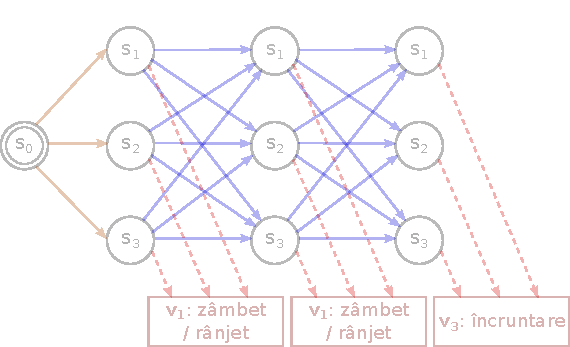
\includegraphics[width=\textwidth]{graphics/viterbi/compute-viterbi/compute-viterbi-none.pdf}}}%
    \only<2>{\framebox{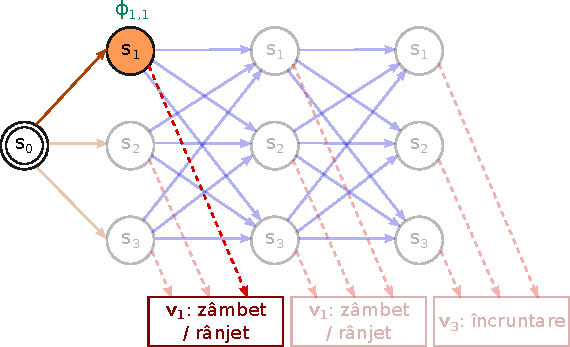
\includegraphics[width=\textwidth]{graphics/viterbi/compute-viterbi/compute-viterbi-11.pdf}}}%
    \only<3>{\framebox{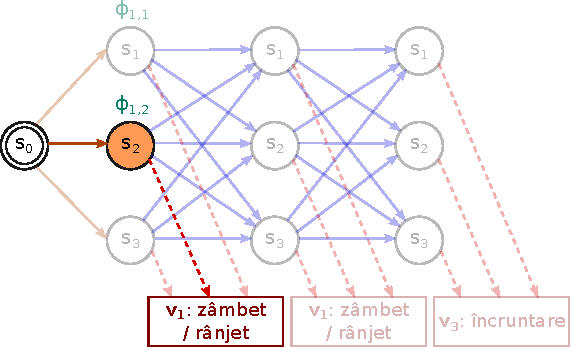
\includegraphics[width=\textwidth]{graphics/viterbi/compute-viterbi/compute-viterbi-12.pdf}}}%
    \only<4>{\framebox{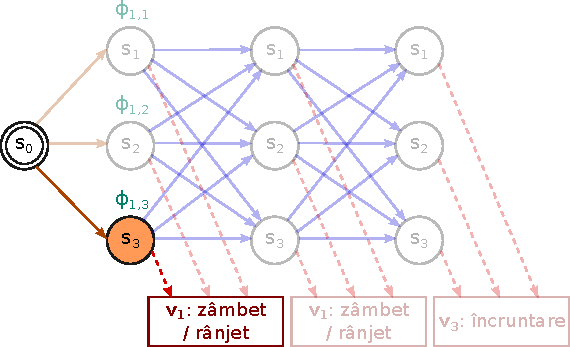
\includegraphics[width=\textwidth]{graphics/viterbi/compute-viterbi/compute-viterbi-13.pdf}}}%
    \only<5>{\framebox{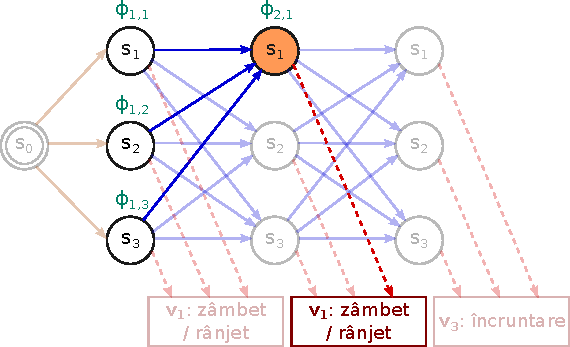
\includegraphics[width=\textwidth]{graphics/viterbi/compute-viterbi/compute-viterbi-21a.pdf}}}%
    \only<6>{\framebox{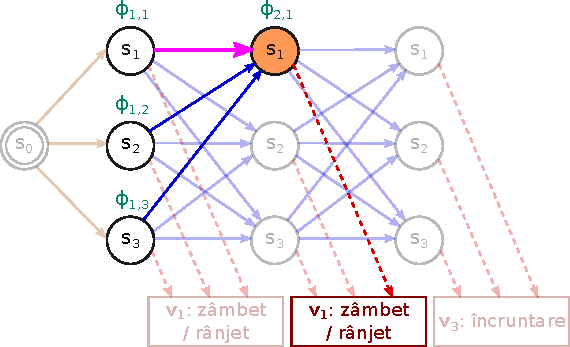
\includegraphics[width=\textwidth]{graphics/viterbi/compute-viterbi/compute-viterbi-21b.pdf}}}%
    \only<7>{\framebox{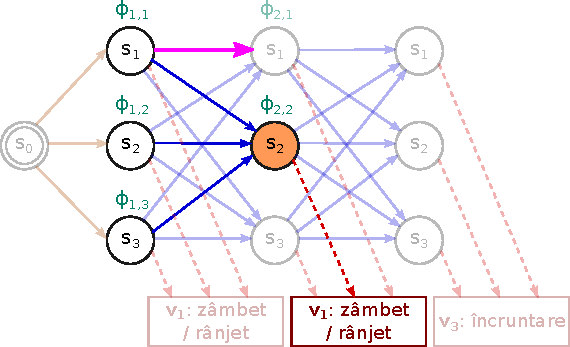
\includegraphics[width=\textwidth]{graphics/viterbi/compute-viterbi/compute-viterbi-22a.pdf}}}%
    \only<8>{\framebox{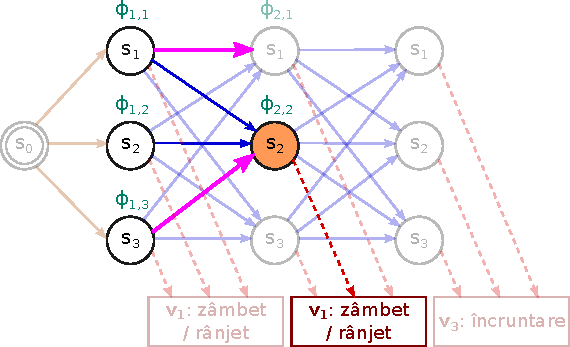
\includegraphics[width=\textwidth]{graphics/viterbi/compute-viterbi/compute-viterbi-22b.pdf}}}%
    \only<9>{\framebox{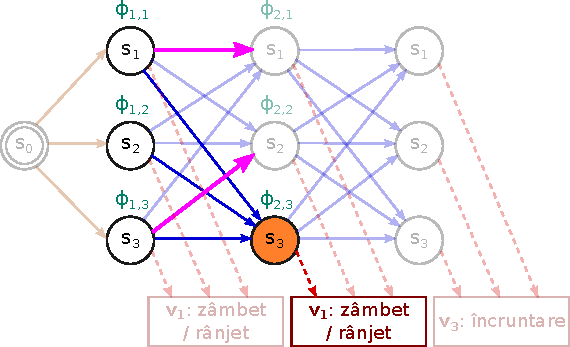
\includegraphics[width=\textwidth]{graphics/viterbi/compute-viterbi/compute-viterbi-23a.pdf}}}%
    \only<10>{\framebox{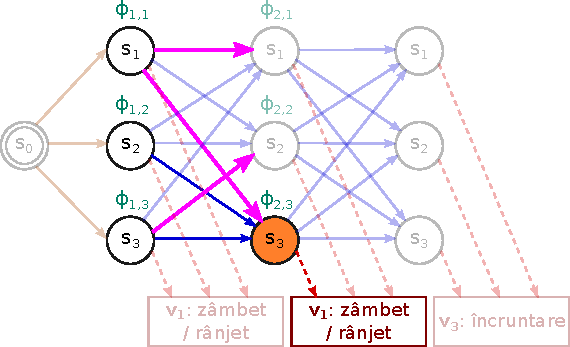
\includegraphics[width=\textwidth]{graphics/viterbi/compute-viterbi/compute-viterbi-23b.pdf}}}%
    \only<11>{\framebox{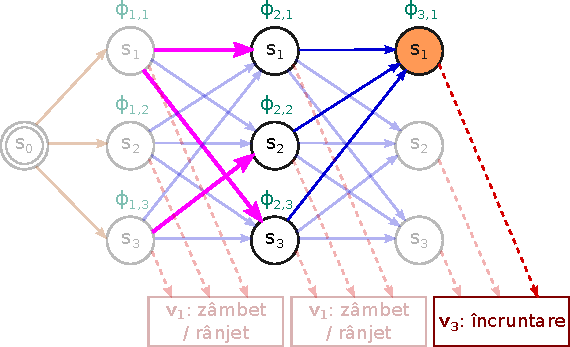
\includegraphics[width=\textwidth]{graphics/viterbi/compute-viterbi/compute-viterbi-31a.pdf}}}%
    \only<12>{\framebox{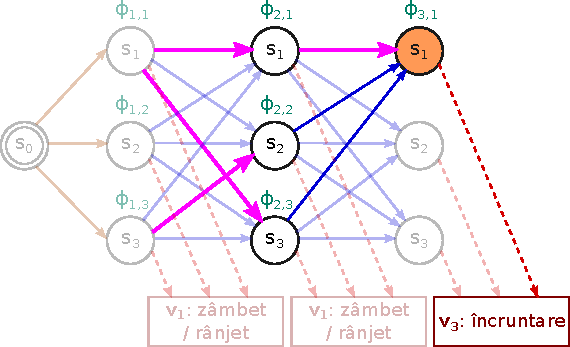
\includegraphics[width=\textwidth]{graphics/viterbi/compute-viterbi/compute-viterbi-31b.pdf}}}%
    \only<13>{\framebox{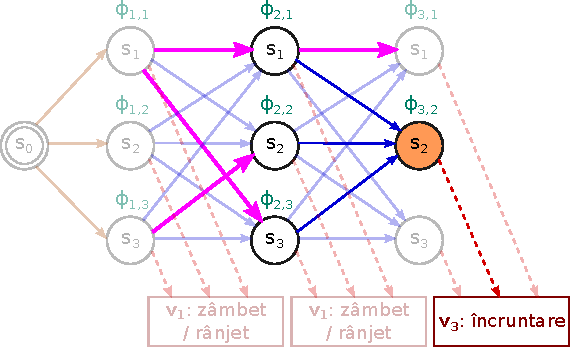
\includegraphics[width=\textwidth]{graphics/viterbi/compute-viterbi/compute-viterbi-32a.pdf}}}%
    \only<14>{\framebox{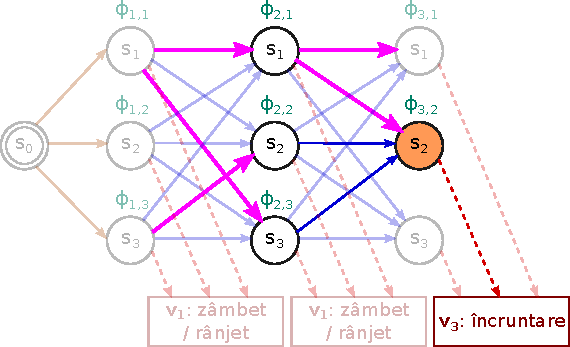
\includegraphics[width=\textwidth]{graphics/viterbi/compute-viterbi/compute-viterbi-32b.pdf}}}%
    \only<15>{\framebox{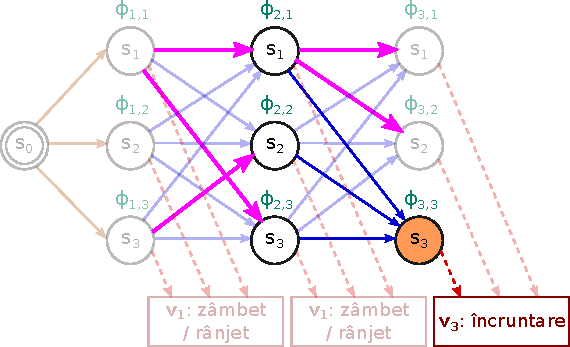
\includegraphics[width=\textwidth]{graphics/viterbi/compute-viterbi/compute-viterbi-33a.pdf}}}%
    \only<16>{\framebox{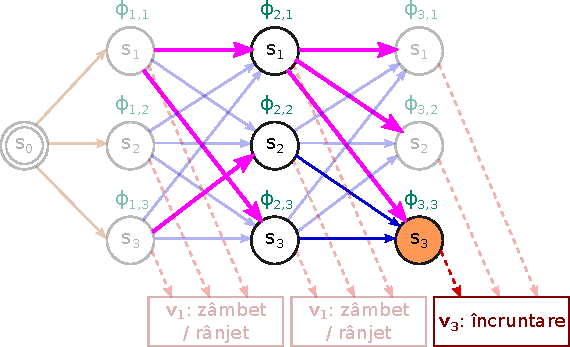
\includegraphics[width=\textwidth]{graphics/viterbi/compute-viterbi/compute-viterbi-33b.pdf}}}%
    \only<17>{\framebox{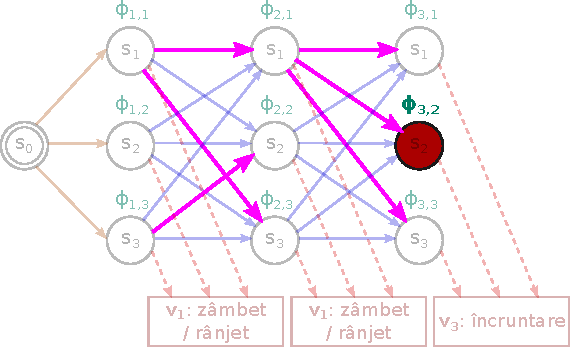
\includegraphics[width=\textwidth]{graphics/viterbi/compute-viterbi/compute-viterbi-3.pdf}}}%
    \only<18>{\framebox{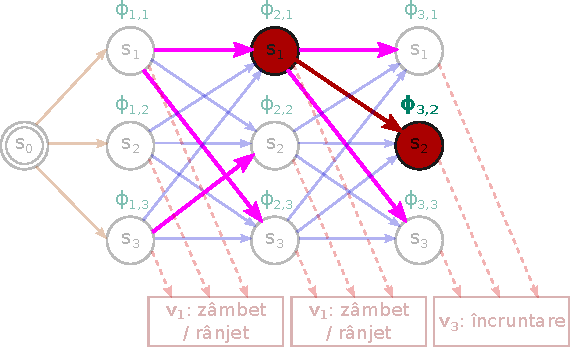
\includegraphics[width=\textwidth]{graphics/viterbi/compute-viterbi/compute-viterbi-2.pdf}}}%
    \only<19>{\framebox{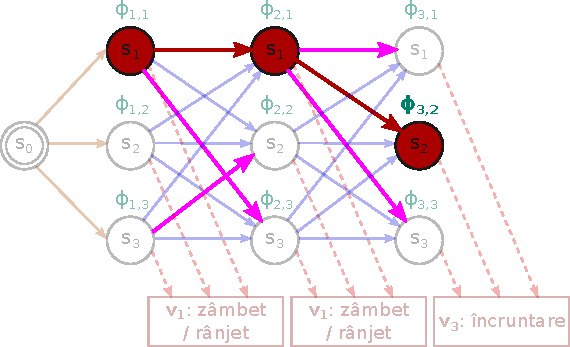
\includegraphics[width=\textwidth]{graphics/viterbi/compute-viterbi/compute-viterbi-1.pdf}}}%
    \column{0.30\textwidth}%
    \only<2>{%
      \begin{equation*}
        \begin{split}
          \scriptstyle \phi_{1,1} & \scriptstyle  = \log(\pi_{1}) + \log(b_{1,1})
      \end{split}
    \end{equation*}
    \vspace*{2em}
    \begin{equation*}
      \begin{split}
        \scriptstyle \psi_{1,1} & \scriptstyle  = 0
      \end{split}
    \end{equation*}
    }\only<3>{%
      \begin{equation*}
      \begin{split}
        \scriptstyle \phi_{1,2} & \scriptstyle  = \log(\pi_{2}) + \log(b_{2,1})
      \end{split}
    \end{equation*}
    \vspace*{2em}
    \begin{equation*}
      \begin{split}
        \scriptstyle \psi_{1,2} & \scriptstyle  = 0
      \end{split}
    \end{equation*}
    }\only<4>{%
      \begin{equation*}
      \begin{split}
        \scriptstyle \phi_{1,3} & \scriptstyle  = \log(\pi_{3}) + \log(b_{3,1})
      \end{split}
    \end{equation*}
    \vspace*{2em}
    \begin{equation*}
      \begin{split}
        \scriptstyle \psi_{1,3} & \scriptstyle  = 0
      \end{split}
    \end{equation*}
    }\only<5>{%
      \begin{equation*}
      \begin{split}
        \scriptstyle \phi_{1,3} & \scriptstyle  = \operatorname{max} \Big\lbrace \\
        \scriptstyle & \scriptstyle \log(\phi_{1,1}) + \log(a_{1,1}),\\ 
        \scriptstyle & \scriptstyle \log(\phi_{2,1}) + \log(a_{2,1}),\\
        \scriptstyle & \scriptstyle \log(\phi_{1,3}) + \log(a_{3,1}) \Big\rbrace \\ 
        \scriptstyle & \scriptstyle + \log(b_{1,1})
      \end{split}
    \end{equation*}
    % \begin{equation*}
    %   \begin{split}
    %     \scriptstyle \psi_{1,3} & \scriptstyle  = \operatorname{argmax} \Big\lbrace \\
    %     \scriptstyle & \scriptstyle \log(\phi_{1,1}) + \log(a_{1,1}),\\ 
    %     \scriptstyle & \scriptstyle \log(\phi_{2,1}) + \log(a_{2,1}),\\
    %     \scriptstyle & \scriptstyle \log(\phi_{1,3}) + \log(a_{3,1}) \Big\rbrace \\
    %   \end{split}
    % \end{equation*}
    }


  \end{columns}
  $\Phi=\begin{bmatrix}
       \scriptstyle \visible<2->{-2.1202} & \scriptstyle \visible<3->{-Inf} & \scriptstyle \visible<4->{-2.1202} \\
       \scriptstyle \visible<5->{-3.7297} & \scriptstyle \visible<7->{-Inf} & \scriptstyle \visible<9->{-4.2205} \\
       \scriptstyle \visible<11->{-6.7254} & \scriptstyle \visible<13->{-5.1567} & \scriptstyle \visible<15->{-5.3391}\end{bmatrix}$ $\Psi=\begin{bmatrix}
       \scriptstyle \visible<2->{0} & \scriptstyle \visible<3->{0} & \scriptstyle \visible<4->{0} \\
       \scriptstyle \visible<6->{1} & \scriptstyle \visible<8->{3} & \scriptstyle \visible<10->{1} \\
       \scriptstyle \visible<12->{1} & \scriptstyle \visible<14->{3} & \scriptstyle \visible<16->{1}\end{bmatrix}$ $Q_{best} = \begin{bmatrix}\visible<19->{1} & \visible<18->{1} & \visible<17->{2}\end{bmatrix}$
     
\end{frame}

\begin{frame}[fragile]
  \frametitle{Algoritmul Viterbi}
  \begin{algorithm}[H]
    \scriptsize
    \caption{Calculul celei mai probabile secvențe $Q_{\text{best}}$}
    \label{alg:viterbi}
    \algsetup{linenosize=\tiny} \algsetup{indent=2.25em}
    \begin{algorithmic}[2]
      \FOR{$i=1$ to $N$}
      \STATE $\phi_{1,i}$ $\leftarrow$ $\log(\pi_{i}) + \log(b_i(o_1))$
      \STATE $\psi_{1,i}$ $\leftarrow$ $0$
      \ENDFOR
      \FOR{$t=2$ to $T$}
      \FOR{$i=1$ to $N$}
      \STATE $\phi_{t,j}$ $\leftarrow$ $[\underset{i}{\operatorname{max}}\; \phi_{t-1,i} +
      log(a_{i,j})] + \log(b_{j}(o_{t}))$
      \STATE $\psi_{t,i}$ $\leftarrow$ $\underset{i}{\operatorname{argmax}}\; \phi_{t-1,i} +
      \log(a_{i,j})$
      \ENDFOR
      \ENDFOR
      \STATE $\log(P(Q_{\text{best}} \vert O, \lambda))$ $\leftarrow$ $\underset{i}{\operatorname{max}}\; \phi_{T,i}$
      \STATE $q_{T_{\text{best}}}$ $\leftarrow$ $\underset{i}{\operatorname{argmax}}\; \phi_{T,i}$
      \FOR{$t=T-1$ to $1$}
      \STATE $q_{t_{\text{best}}}$ $\leftarrow$ $\psi_{t+1}(q_{t+1_{\text{best}}})$
      \ENDFOR
    \end{algorithmic}
  \end{algorithm}
\end{frame}

\begin{frame}
  \frametitle{A venit vremea să scriem cod}
  \begin{enumerate}
  \item Faceți o copie a fișierului \texttt{viterbi\_disc.m.stub} 
    și denumiți-o \texttt{viterbi\_disc.m} (eliminați sufixul \texttt{.stub}).
    \\Veți implementa funcția:\\
    \mcode{function [logP, Q] = viterbi_disc(O,Pi, A, B)}
    \pause
  \item Completați cele două secțiuni.%
    \vspace*{-1em}
    \lstinputlisting{m-files/viterbi.m}
\item Folosiți \mcode{hmm_test} pentru a vă testa codul.
\end{enumerate}
\end{frame}

\part{Demo \& Discussions}

\begin{frame}[t]
	\frametitle{Aplicație de recunoaștere a simbolurilor}
	Features:
	\pause
	\begin{block}{Definire}
		Definire, organizare și vizualizare a unui set de date de simboluri captate prin mișcarea mouse-ului.
	\end{block}
	\pause
	
	\begin{block}{Antrenare}
		Antrenarea unui motor de recunoaștere a simbolurilor prin metoda MMA.
	\end{block}
	\pause
	
	\begin{block}{Recunoaștere}
		Recunoașterea unui nou simbol si vizualizarea unor metrici de clasificare.
	\end{block}
	\pause
	
	\begin{block}{}
		Simboluri default incluse: \textbf{\emph{săgeată stânga, săgeată dreapta, cerc, pătrat, infinit}}
	\end{block}
\end{frame}

\begin{frame}[t]
	\frametitle{Aplicație de recunoaștere a simbolurilor - Preview}	
	
	\begin{figure}
  		\centering
		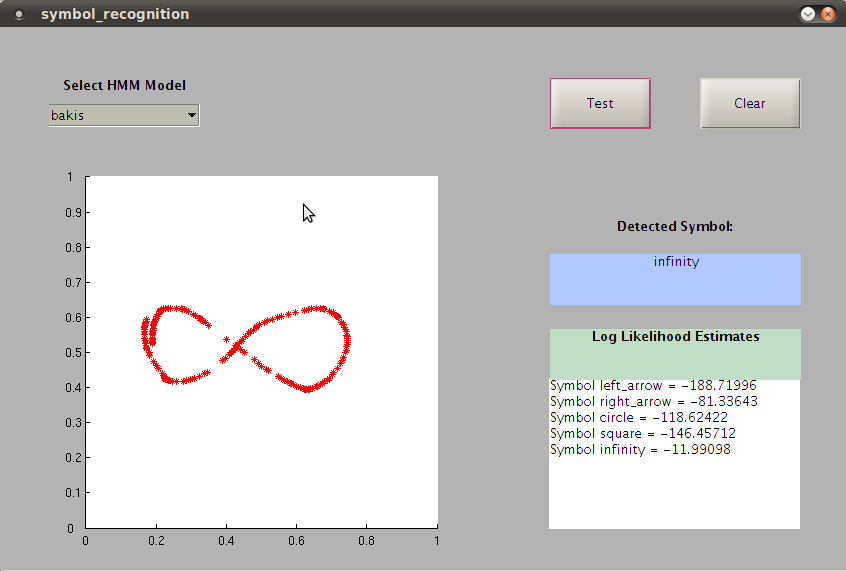
\includegraphics[height=0.70\textheight]{graphics/demo-app/infinity.png}
		\caption{\tiny{O vizualizare cu GUI-ul aplicației de recunoaștere a simbolurilor}}
		\label{fig:baum-welch-alg}
  	\end{figure}	
\end{frame}

\begin{frame}[t]
	\frametitle{Aplicație de recunoaștere a simbolurilor - Abordare}
	Adapted from \citep{yang1994hidden}.\\%
	\vspace*{0.5em}%
	\only<1>{\centering 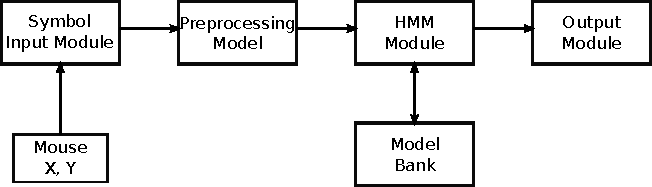
\includegraphics[width=0.80\textwidth]{graphics/demo-app/symbol-app-architecture-1.pdf}}%
	\only<2>{\centering 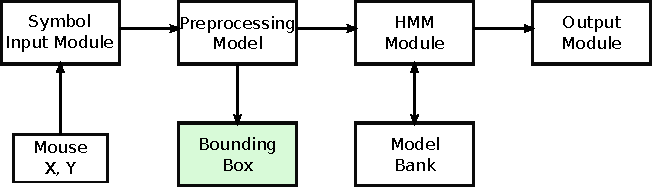
\includegraphics[width=0.80\textwidth]{graphics/demo-app/symbol-app-architecture-2.pdf}}%
	\only<3>{\centering 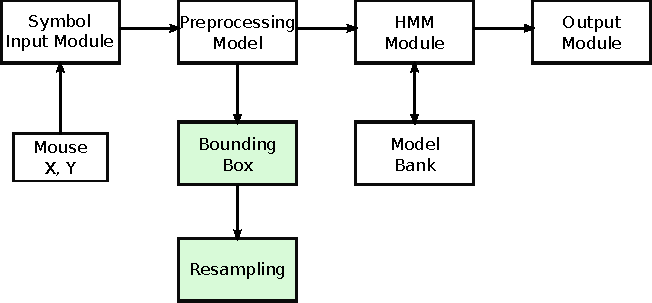
\includegraphics[width=0.80\textwidth]{graphics/demo-app/symbol-app-architecture-3.pdf}}%
	\only<4>{\centering 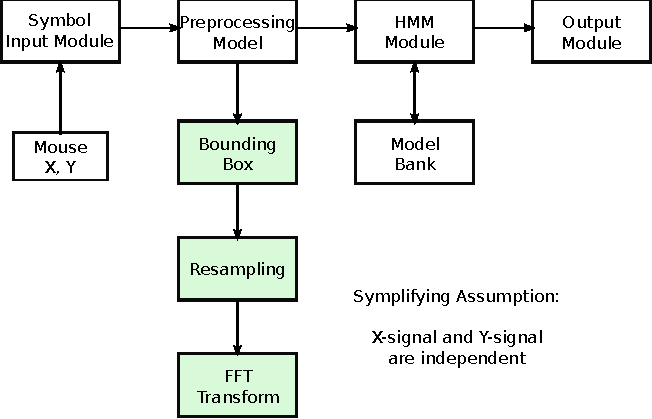
\includegraphics[width=0.80\textwidth]{graphics/demo-app/symbol-app-architecture-4.pdf}}%
	
\end{frame}

\begin{frame}
	\frametitle{Aplicație de recunoaștere a simbolurilor - Abordare}
	Adaptare după \citep{yang1994hidden}.
	
	\begin{block}{Structura MMA}
		$N$(număr de stări) = 8\\
		2 variabile observabile de tip discrte per stare - $coef_{FFT}(x)$, $coef_{FFT}(y)$\\
		$M$(număr de valori pentru fiecare variabilă observabilă) = 256\\
		Modelul de tranziție:\\
		\begin{itemize}
			\item Bakis
			\item Ergodic
		\end{itemize}
	\end{block}
\end{frame}

\begin{frame}
	\frametitle{Aplicație de recunoaștere a simbolurilor - Abordare}
	
	Procedură de recunoaștere:
	\begin{enumerate}
		\item Construim și antrenăm câte un MMA pentru fiecare simbol în parte
		\vspace*{0.5em}
		\pause
		\item Folosim un set de date (simboluri) de validare pentru a stabili \emph{praguri} de recunoaștere, i.e. 
				dacă probabilitatea secvenței observate este prea mică pentru fiecare MMA, marcăm simbolul drept 
				\emph{necunoscut}
		\vspace*{0.5em}
		\pause
		\item Recunoaștere:
			\begin{itemize}
				\item Calculăm $P(O \vert \lambda_i)$ pentru fiecare MMA construit pentru simbolurile 
				$i=1,\cdots,nr\_simboluri$
				\item Alegem $\max(P(O \vert \lambda_i))$ ca și simbol candidat. 
				Daca $P(O \vert \lambda_i) > prag_i$, atunci am recunoscut \emph{simbolul i}, 
				altfel marcăm \emph{necunoscut}
			\end{itemize}
	\end{enumerate}
	
\end{frame}

\begin{frame}[t]
	\frametitle{Aplicație de recunoaștere a simbolurilor - Rezultate}
	\scriptsize
	\begin{block}{Mărime set de date}
		\textbf{5} simboluri: \textbf{\emph{săgeată stânga, săgeată dreapta, cerc, pătrat, infinit}}\\
		\textbf{100} exemple per simbol: \textbf{50} antrenare, \textbf{10} validare, \textbf{40} testare
	\end{block}
	\normalsize
	
	\begin{columns}[T]
		\column{0.5\textwidth}
		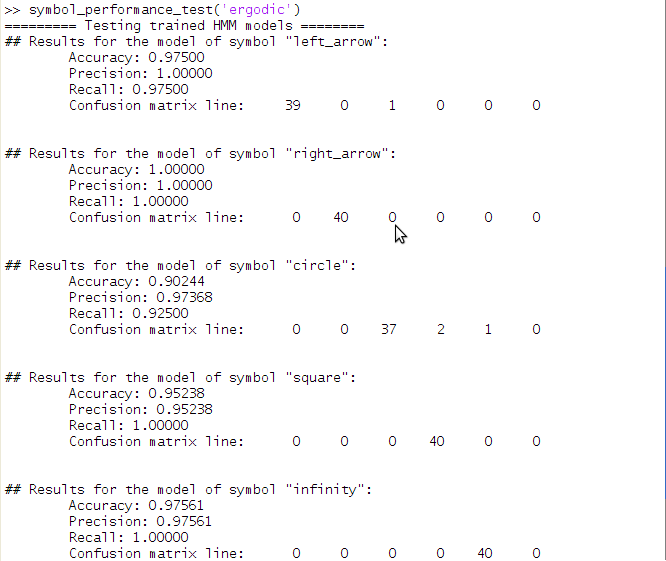
\includegraphics[width=\textwidth]{graphics/demo-app/results-ergodic.png}
		\column{0.5\textwidth}
		\includegraphics[width=\textwidth]{graphics/demo-app/results-bakis.png}
	\end{columns}
\end{frame}
\begin{frame}
  \frametitle{Modele Markov Complet}
  \begin{block}{Modele Markov Complet}
    Un lanț Markov se numește \alert{complet} dacă din orice stare se poate ajunge în oricare altă stare direct.\\
    Matricea de tranziție nu are nicio valoare nulă.
  \end{block}
  \vspace*{1em}
  \begin{center}
    \includegraphics[width=0.4\textwidth]{graphics/other-hmm/full.pdf}
  \end{center}
\end{frame}


\begin{frame}
  \frametitle{Modele Markov Ergodice}
  \begin{block}{Modele Markov Ergodice}
    Un lanț Markov se numește \alert{ergodic} dacă din orice stare se poate ajunge în oricare altă stare (nu neaparat într-o singură mutare).\\
    Lanțurile Markov ergodice se mai numesc și \emph{ireductibile}.
  \end{block}
  \vspace*{1em}
  \begin{center}
    \includegraphics[width=0.8\textwidth]{graphics/other-hmm/ergodic.pdf}
  \end{center}
\end{frame}

\begin{frame}
  \frametitle{Modelul Bakis}
  \begin{block}{Modele Markov Bakis (stânga $\longrightarrow$ dreapta)}
    Un model \alert{Bakis} este unul în care nu este permisă tranziția
    dintr-o stare către o altă stare cu un indice mai mic.
  \end{block}
  \vspace*{1em}
  \begin{center}
    \includegraphics[width=0.8\textwidth]{graphics/other-hmm/left-to-right.pdf}
  \end{center}
\end{frame}

\begin{frame}
  \frametitle{Alte tipuri de MMA}
  \begin{itemize}
  \item modele Markov cu memorie mixtă \citep{Saul:1999:MMM:326214.325611}
    \begin{itemize}
    \item scalează mai bine cu secvențe de lungime mare
    \item utile în: modelarea vizitării paginilor web
    \end{itemize}
    \vspace*{.5em}
  \item modele Markov ascunse de durată variabilă \citep{rabiner1989tutorial}
    \begin{itemize}
    \item utile în: recunoașterea cuvintelor scrise cursiv de mână \citep{chen1995variable}
    \end{itemize}
    \vspace*{.5em}
  \item modele Markov ascunse factoriale \citep{Ghahramani97factorialhidden}
    \begin{itemize}
    \item mai multe variabile de stare
    \item putere de modelare mai mare
    \item algoritmi exacți intractabili
    \end{itemize}
    \vspace*{.5em}
  \item modele Markov ascunse ierarhice \citep{fine1998hierarchical}
    \begin{itemize}
    \item utile în: recunoașterea scrisului de mână cursiv
    \end{itemize}
  \end{itemize}
\end{frame}
\section{Discussions and Recap}
\label{sec:final}

\begin{frame}
  \frametitle{Summary}
  \begin{itemize}
  \item HMM are useful for temporal sequence problems
    \pause
  \item there are 3 fundamental problems for HMMs:
    \begin{itemize}
    \item<3-> given an HMM, estimating the probability of an observed sequence
      \visible<6->{\structure{Forward-Backward Algorithm}}
    \item<4-> given observed data, estimating the parameters of an HMM
      \only<7->{\structure{Baum-Welch Algorithm}}
    \item<5-> uncovering the hidden states
      \visible<8->{\structure{Viterbi Algorithm}}
    \end{itemize}

  \end{itemize}
\end{frame}
\section[References]{}
\label{sec:references}
\begin{frame}[allowframebreaks]{References}
  \bibliographystyle{apalike}
  \bibliography{hmm.bib}
\end{frame}

\section[Thanks]{}
\label{sec:thanks}

\begin{frame}{Thank you!}
  
\end{frame}




\end{document}

